\documentclass[../main/main.tex]{subfiles}
\begin{document}

% \dominitoc
% \faketableofcontents
% \dominilof
% \fakelistoffigures
% \dominilot
% \fakelistoftables

\chapter{Pr\'esentation des sondages}\label{ch:surveys}
\epigraph{\openquote\textit{Simplicity is the final achievement. After one has
        played notes and more notes, it is simplicity that emerges as the
crowning reward of art.}\closequote}{\textsc{Chopin}}

\vfill
Comme nous en avons discuté initialement (voir Chapitre~\ref{ch:cosmo}), les
SNe~Ia sont un excellent outil pour sonder les propriétés de l'Univers. Depuis
la découverte de son expansion accélérée \citep{riess1998, perlmutter1999}, de
nombreux relevés cosmologiques visant à acquérir des données de SNe~Ia ont vu le
jour.

La diversité des régions d'Univers à sonder implique des stratégies variées, et
chaque sondage s'inscrit dans un contexte particulier avec ses propres
instruments, caractéristiques et objectifs scientifiques. S'ils permettent
ensemble d'améliorer la statistique de ces mesures, leurs différentes approches
de relevé sont parfois notables et il convient de comprendre leurs ancrages pour
en comprendre les spécificités.

Ainsi nous présentons dans ce chapitre les sondages dont nous utilisons les
données ou qui apparaissent dans cette thèse. Les cinq premiers constituent
notre échantillon de base, alors que les deux derniers ont une présence limitée
dans notre étude. Un comparatif des caractéristiques des sondages est présenté
Tableau~\ref{tab:sondcomp}.

\vfill

\newpage
\vfill
\minitoc
\vfill
\newpage

\section{The Nearby Supernova factory}\label{sec:snf}
\subsection{Introduction}\label{ssec:snfintro}

La collaboration \textit{The Nearby Supernova factory}
\citep[SNfactory,][]{aldering2002} est créée peu de temps après la découverte de
l'expansion accélérée de l'Univers \citep{riess1998, perlmutter1999} avec pour
but un suivi spectrophotométrique d'une précision d'environ 1\% de SNe~Ia
proches. Un de ses objectifs est de peupler la partie basse du diagramme de
\textsc{Hubble} ($0,03 < z < 0,08$) pour permettre son ancrage à bas redshift,
qui ne contenait alors qu'une vingtaine de SNe~Ia \citep{hamuy1996}. Par sa
nature purement spectrophotométrique, la mission tente également d'étudier
précisément les propriétés des SNe~Ia. En effet, une étude fine spectrale est
nécessaire afin de mieux comprendre leur diversité, mettre en évidence
différentes populations de supernovae et améliorer leur standardisation grâce à
une meilleure compréhension de leurs variabilités et ainsi réduire les erreurs
systématiques dans les mesures de paramètres cosmologiques. Avec les données de
SNf, \cite{rigault2020} ont montré une forte corrélation entre le traceur LsSFR
(Section~\ref{sssec:lssfr}) et les propriétés des SNe~Ia, établissant la base de
notre analyse sur l'âge des SNe~Ia.

\subsection{Détection des supernovae}\label{ssec:snfdetec}

Le programme a été sujet à plusieurs évolutions au cours de son fonctionnement,
notamment pour la découverte de nouveaux candidats. Ce sont d'autres télescopes
qui alertent la communauté. En premier lieu, jusqu'à fin 2008, le télescope de
\SI{1,2}{m} du Mont Palomar en Californie \citep{rabinowitz2003} scannait
\SI{500}{deg^2} du ciel chaque soir avec la caméra QUEST de 112 capteurs CCD,
observant en bandes $UBVRI$. À partir de 2010, les candidats de SNe proviennent
d'une coopération avec \textit{Palomar Transient Factory}
\citep[PTF,][]{law2009} et de données publiques. La caméra QUEST fut ensuite
déplacée à La Silla au Chili \citep[LSQ,][]{hadjiyska2012} pour reprendre,
mi-2012, l'activité de recherche de SNe pour SNfactory. Les candidats potentiels
sont à chaque fois programmés pour observation spectroscopique afin de les
identifier en tant que SNe~Ia et décider de leur suivi selon des critères de
qualité (nombre de points de mesure, proche et avant du maximum,
non-contamination par la luminosité de la Lune notamment). Les transmissions des
filtres $UBVRI$ de La Silla issues du service de profils de filtres du
\textit{Spanish Virtual Observatory} \citep[SVO\footnote{
    \href{http://svo2.cab.inta-csic.es/theory/fps/index.php?asttype=astro}
{http://svo2.cab.inta-csic.es/theory/fps/index.php?asttype=astro}},][]
{rodrigo2020} sont tracées Figure~\ref{fig:snfbands}, et un exemple de courbe de
lumière d'une SN identifiée par SNf est donné Figure~\ref{fig:snflc}.

% \begin{figure}[ht]
%     \centering
%     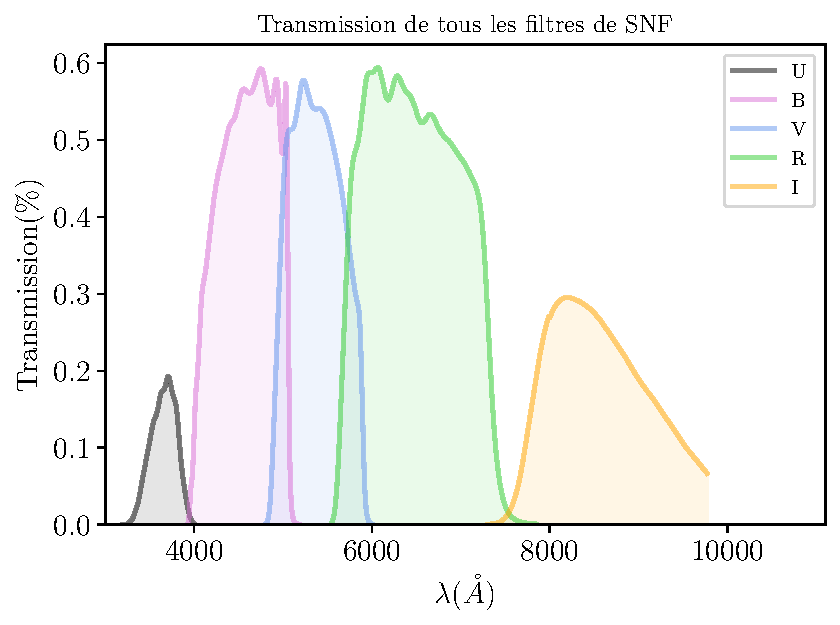
\includegraphics[width=.8\linewidth]{bands_SNF.pdf}
%     \caption{Transmissions des filtres de La Silla utilisés par SNF.}
%     \label{fig:snfbands}
% \end{figure}
% \begin{figure}[ht]
%     \centering
%     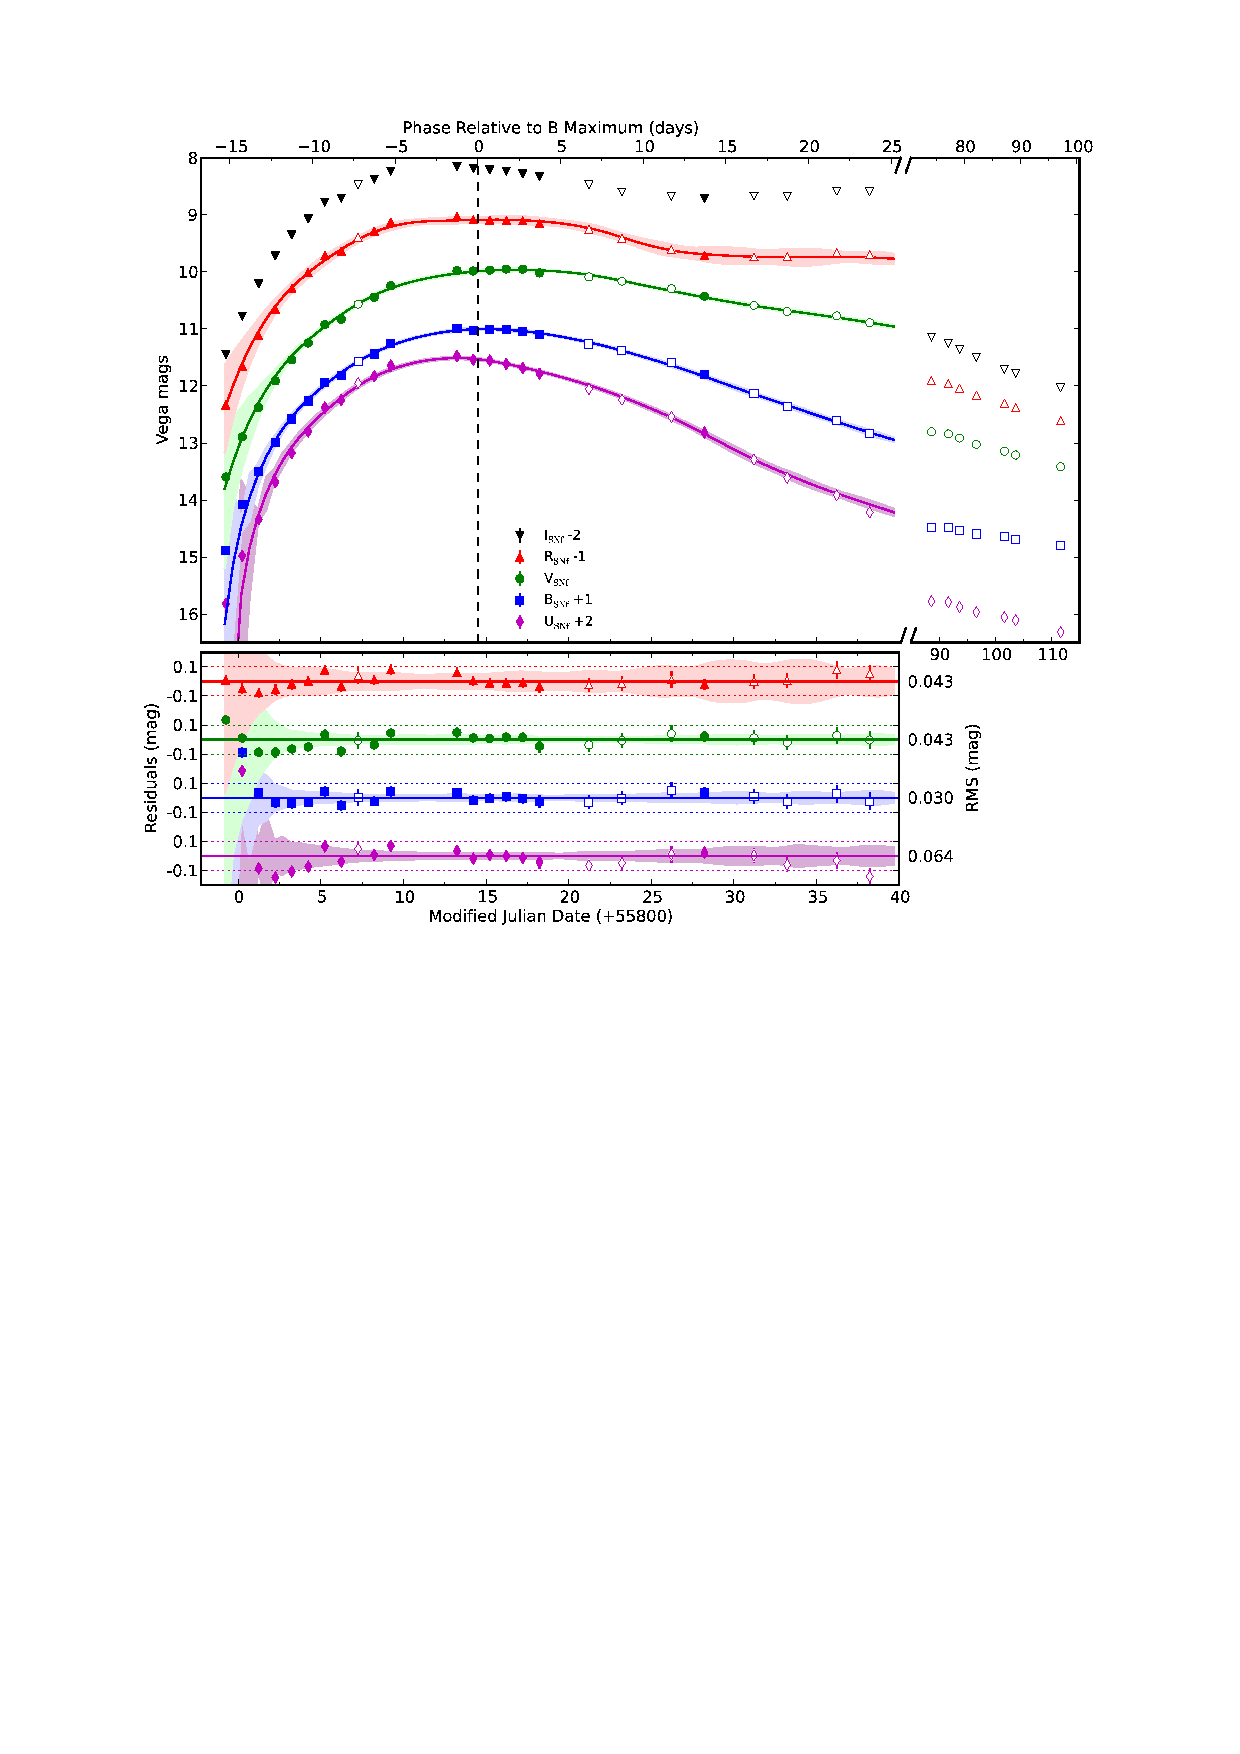
\includegraphics[width=.8\linewidth,
%                      trim={2cm 14cm 2.5cm 2cm},
%                      clip]{2011fe_lightcurves}
%     \caption{Courbes de lumières en bandes $UBVRI$ de la SNe~Ia confirmée
%     2011fe. Figure de~\cite{pereira2013}.}
%     \label{fig:snflc}
% \end{figure}

\begin{figure}[ht]
    \centering
    \begin{subfigure}[]{.44\linewidth}
        \centering
        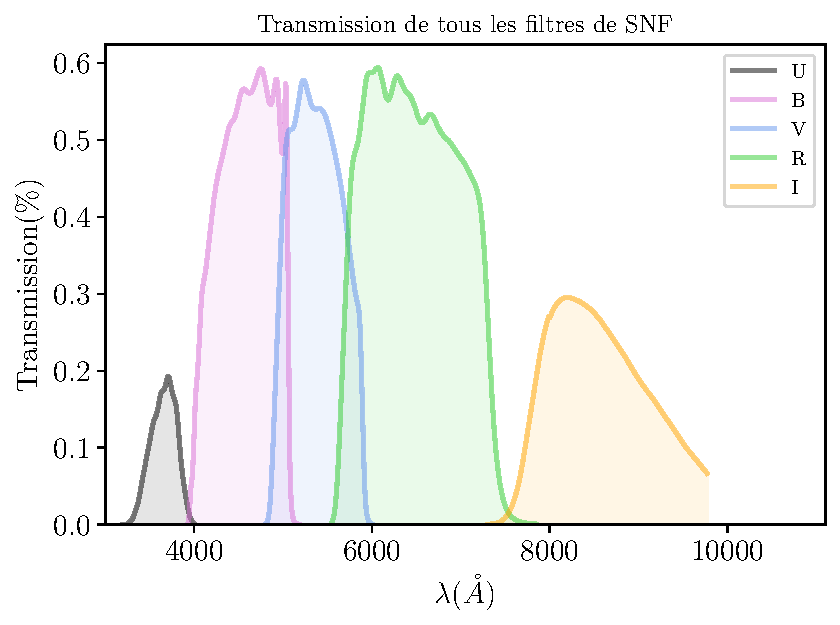
\includegraphics[width=\linewidth]{bands_SNF.pdf}
        \caption{Transmissions des filtres utilisés par l'observatoire La Silla,
        collaborant avec SNf pour la recherche de candidats. Données issues du
    SVO \citep{rodrigo2020}.}
        \label{fig:snfbands}
    \end{subfigure}
    \hfill
    \begin{subfigure}[]{.54\linewidth}
        \centering
        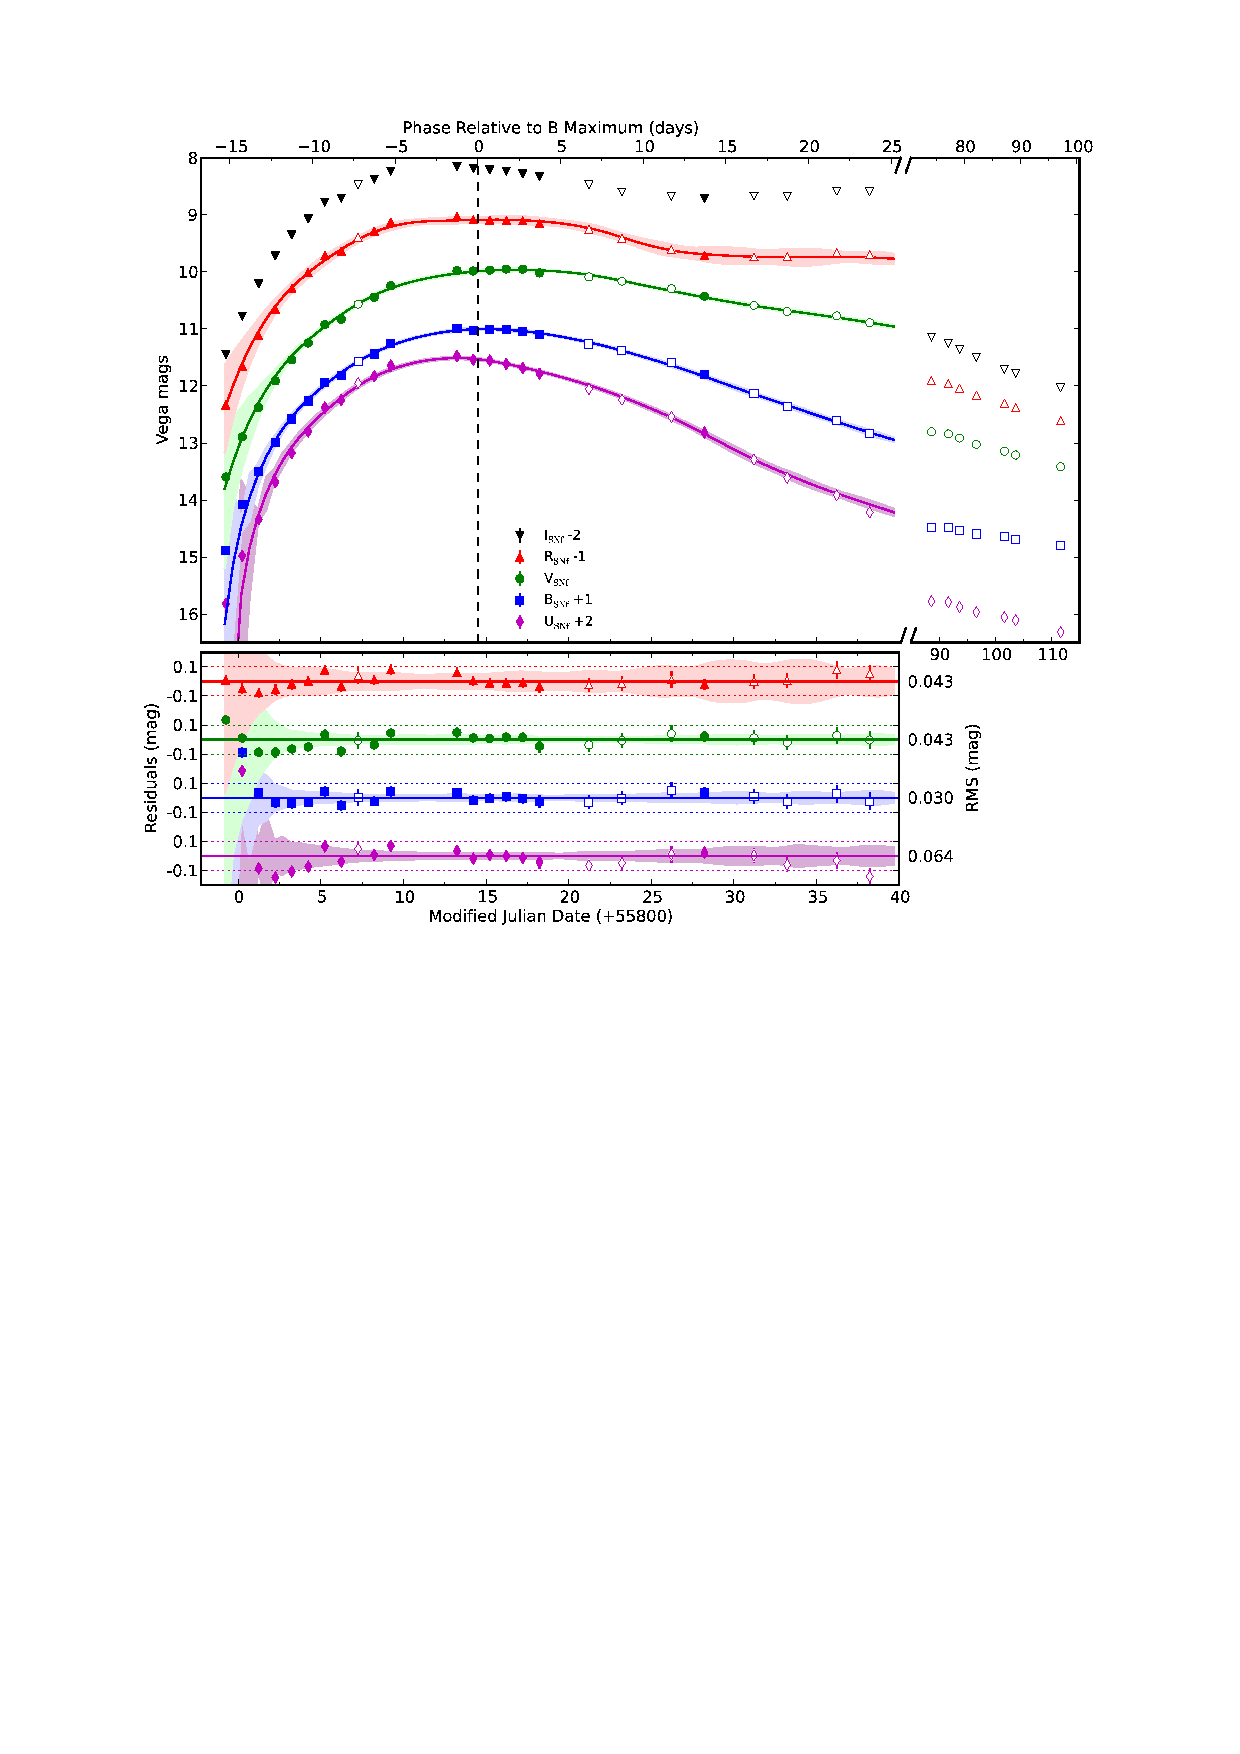
\includegraphics[width=\linewidth,
                         trim={2cm 18.75cm 2.5cm 2.0cm},
                         clip]{2011fe_lightcurves}
        \caption{Courbe de lumière en bandes $UBVRI$ de la SN~Ia confirmée
            SN2011fe avec ajustement par \texttt{SALT2} (ligne pleine et bande
        pour son erreur). Figure de~\cite{pereira2013}.}
        \label{fig:snflc}
    \end{subfigure}
    \caption{Caractéristiques du sondage SNF.}
\end{figure}

\subsection{Suivi spectrophotométrique}\label{ssec:snfspectro}

Le typage spectroscopique, quand il n'a pas déjà été réalisé par d'autres
collaborations ayant donné l'alerte, est assuré par le \textit{SuperNovae
Integral Field Spectrograph} \citep[SNIFS,][]{lantz2004} du télescope de
l'Université d'Hawaii de \SI{2,2}{m} au sommet du Mauna Kea, mis en service en
2004. Il s'avère plus efficace qu'un typage photométrique qui nécessite
plusieurs observations dans différents filtres de couleur, bien que ces
dernières soient plus simples à mettre en place.

Ce spectrographe dit «~à champ intégral~» récolte des «~cubes~», des données en
3 dimensions, deux spatiales représentant un point dans le ciel plus une
dimension de longueur d'onde. Chaque point de ce relevé se nomme
\textit{spaxel}, pour «~spatial picture element~», et ensemble forment une
grille de 15 $\times$ 15 pour un champ de vue total de
$\ang{;;6,4}\times\ang{;;6,4}$ dans deux longueurs d'ondes~: une voie bleue
($B$) de 3200 à \SI{5200}{\angstrom} et une voie rouge ($R$) de 5100 à
\SI{10000}{\angstrom}.

En plus de cette voie, SNIFS possède une voie photométrique utilisant 5 filtres
$ugriz$ pour suivre l'absorption atmosphérique, et une voie de guidage avec un
filtre $V$ pour aider le télescope à la focalisation. Le champ de ces caméras
est de \ang{;4,5;} $\times$ \ang{;9;}.

\subsection{Description des données conservées}\label{ssec:snfdata}

De 2004 à 2013, SNfactory a classifié 1364 objets dont plus de 1000 supernovae,
observé 645 SNe~Ia au moins une fois et en a suivi plus de 271 SNe~Ia, avec au
moins 5 points de mesure \citep{copin2013}.

Sur celles-ci, 198 ont des mesures satisfaisant les contraintes nécessaires à
l'établissement de leur courbe de lumière et sont associées à une galaxie hôte
permettant de déterminer leur redshift. Afin de déterminer efficacement les
propriétés locales de leur environnement, seules les SNe entre $z = 0,02$ et $z
= 0,08$ sont conservées, amenant l'échantillon à 160 objets.

Les données pour lesquelles les images des galaxies hôtes dans les bandes
photométriques $g$ et $i$ sont contaminées par la luminosité des SNe sont
également rejetées. En effet, ces bandes s'avèrent nécessaires à la
détermination de la masse stellaire de la galaxie. Cette coupe réduit
l'échantillon à 147 objets.

Les SNe considérées comme trop «~anormales~» sont exclues car supposées non
représentatives de la population générale que l'on souhaite étudier. Elles sont
au nombre de 6.

Finalement, parmi ces 141, ne sont conservées que celles provenant directement
des collaborations internes, c'est-à-dire celles de SNf, PTF et LSQ.
L'échantillon final est alors de 114 données. L'ensemble de ces critères de
sélection est résumé Tableau~\ref{tab:snfcuts}.

\begin{table}[ht]
    \centering
    \caption{Critères de sélection des SNe~Ia suivies par SNfactory.}
    \label{tab:snfcuts}
    \begin{tabular}{lc}
        \toprule
        Critères de sélection           & Nb de SNe~Ia \\
        \midrule
        Suivies                         & 271 \\
        Courbe de lumière + hôte        & 198 \\
        $0,02 < z < 0,08$               & 160 \\
        Hôte $g$ et $i$ non contaminées & 147 \\
        SNe~Ia «~normales~»             & 141 \\
        SNf LSQ ou PTF seulement        & 114 \\
        \bottomrule
    \end{tabular}
\end{table}

Grâce au suivi spectroscopique de tous les candidats à $r \lesssim
\SI{19,5}{mag}$ et ces limitations en redshift, ces données sont considérées
comme étant limitées en volume, c'est-à-dire un tirage aléatoire des populations
sous-jacentes de SNe~Ia. On présente Figure~\ref{fig:snfhist} les distributions
de redshift, étirement et couleur de ces 114 SNe~Ia.

\begin{figure}[ht]
    \centering
    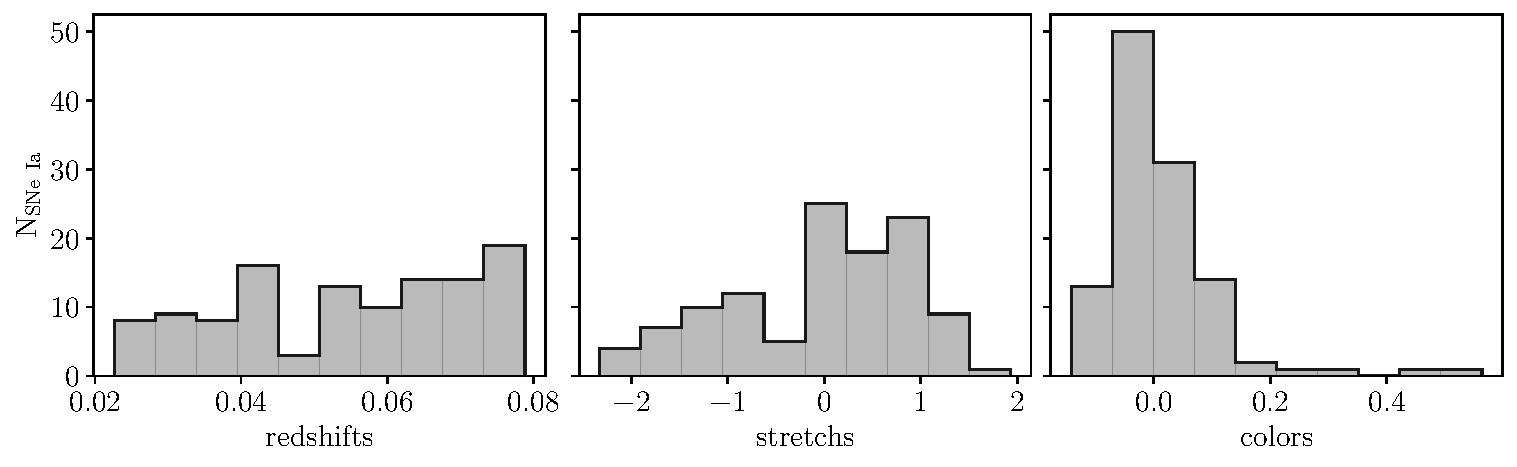
\includegraphics[width=\linewidth]{hist_SNF_zxc.pdf}
    \caption[Distributions des paramètres de redshift, étirement et couleur de
    SNf]{Distributions des paramètres de redshift (à gauche), d'étirement (au
    milieu) et de couleur (à droite) pour les 114 données de SNfactory.}
    \label{fig:snfhist}
\end{figure}

\section{Sloan Digital Sky Survey}\label{sec:sdss}
\subsection{Introduction}\label{ssec:sdssintro}

Le \textit{Sloan Digital Sky Survey} \citep[SDSS,][]{frieman2008, sako2008,
sako2018} est un sondage astronomique majeur qui a débuté en 2000 et est encore
actif
aujourd'hui\footnote{\href{https://www.sdss5.org/}{https://www.sdss5.org/}}. Le
programme se divise en cinq phases d'observation de différents objets
astrophysiques, de simples étoiles aux grandes structures de l'Univers. La
partie supernova du sondage est une des trois composantes de la seconde phase et
s'étend de 2005 à 2008~; ce sera la seule que nous détaillerons ici. Son
objectif principal est de répondre au manque de données astrophysiques à
redshifts intermédiaires par rapport aux sondages de l'époque~: l'intervalle de
redshifts sondés est entre $0,05 \lesssim z \lesssim 0,45$, partie encore peu
peuplée en 2005. À cela s'ajoute la volonté de réduire les limitations
systématiques des autres programmes afin d'améliorer les contraintes sur les
propriétés de l'énergie sombre, par l'utilisation de sa combinaison unique de
couverture céleste, précision photométrique et grande sensibilité. Ceci est
rendu possible grâce à la première phase du sondage qui a apporté une large base
de données d'images de références, de catalogues d'objets et de calibration
photométrique.

\subsection{Détection des supernovae}\label{ssec:sdssdetec}

La stratégie d'observation de SDSS se concentre sur \SI{300}{deg^2} du ciel
faiblement affectée par l'extinction galactique, nommée Bande 82, en y répétant
l'acquisition. Elle est réalisée grâce au télescope optique dédié de \SI{2,5}{m}
\citep{gunn2006} à Apache Point au Nouveau Mexique, couplé à une caméra CCD
\citep{gunn1998} à 5 filtres optiques \citep[$ugriz$,][]{fukugita1996} qui
tournent avec une cadence relativement haute, environ une acquisition toutes les
4 à 5 nuits. Les transmissions de ces filtres sont tracées
Figure~\ref{fig:sdssbands}. Le procédé d'acquisition est similaire à celui de
SNf, étant tous les deux des sondages à recherche glissante~: différentes images
du ciel sont comparées pour détecter les phénomènes transitoires et créer des
courbes de lumière. Cette stratégie a permis à SDSS de détecter la majeure
partie de ses SNe bien avant leur maximum d'émission (pour $z \lesssim 0,3$)
avec des courbes bien échantillonnées en plusieurs bandes photométriques (cf.
Figure~\ref{fig:sdsslc}).

\begin{figure}[ht]
    \centering
    \begin{subfigure}[]{.49\linewidth}
        \centering
        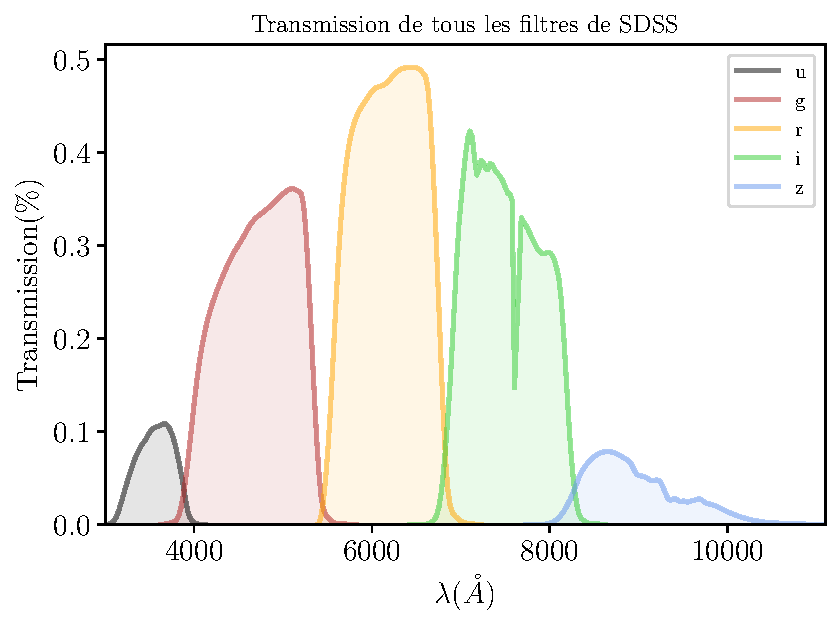
\includegraphics[width=\linewidth]{bands_SDSS.pdf}
        \caption{Transmissions des filtres utilisés par le sondage SDSS. Données
        tirées du SVO \citep{rodrigo2020}.}
        \label{fig:sdssbands}
    \end{subfigure}
    \begin{subfigure}[]{.49\linewidth}
        \centering
        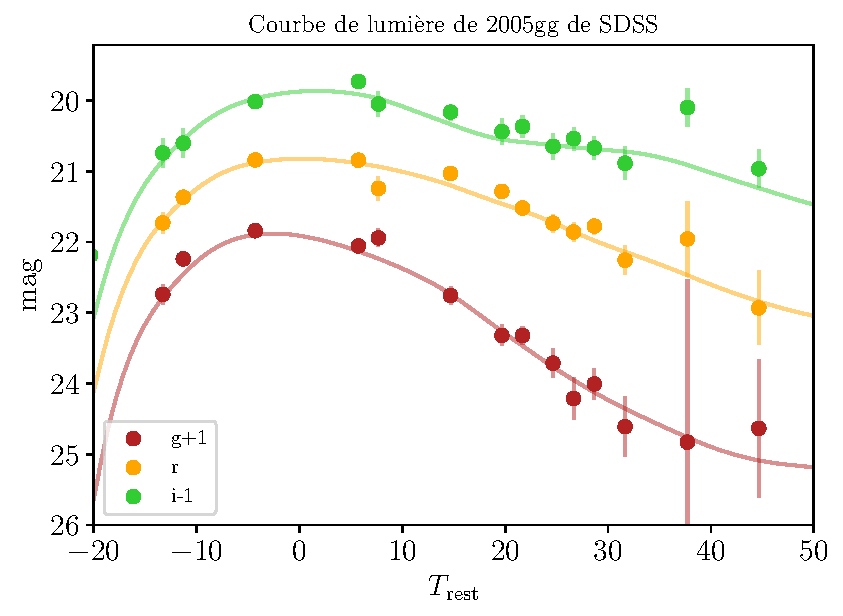
\includegraphics[width=\linewidth]{lc_2005gg.pdf}
        \caption{Courbe de lumière en bandes $gri$ de la SN~Ia
            confirmée 2005gg, à $z = 0,230$. Figure produite avec les données du
        sondage et de l'analyse Pantheon \citep{scolnic2018}.}
        \label{fig:sdsslc}
    \end{subfigure}
    \caption{Caractéristiques du sondage SDSS.}
\end{figure}

% \begin{figure}[ht]
%     \centering
%     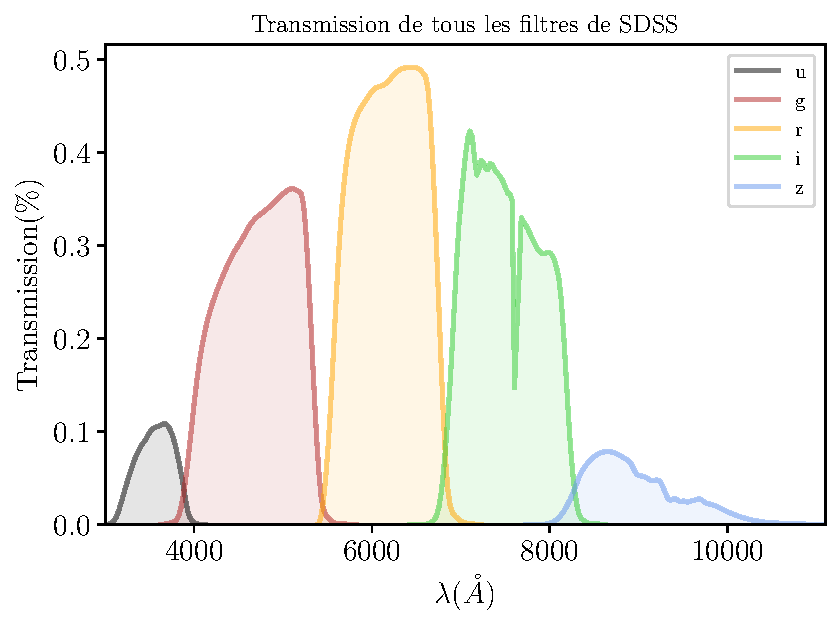
\includegraphics[width=.8\linewidth]{bands_SDSS.pdf}
%     \caption{Transmissions des filtres de SDSS.}
%     \label{fig:sdssbands}
% \end{figure}
% 
% \begin{figure}[ht]
%     \centering
%     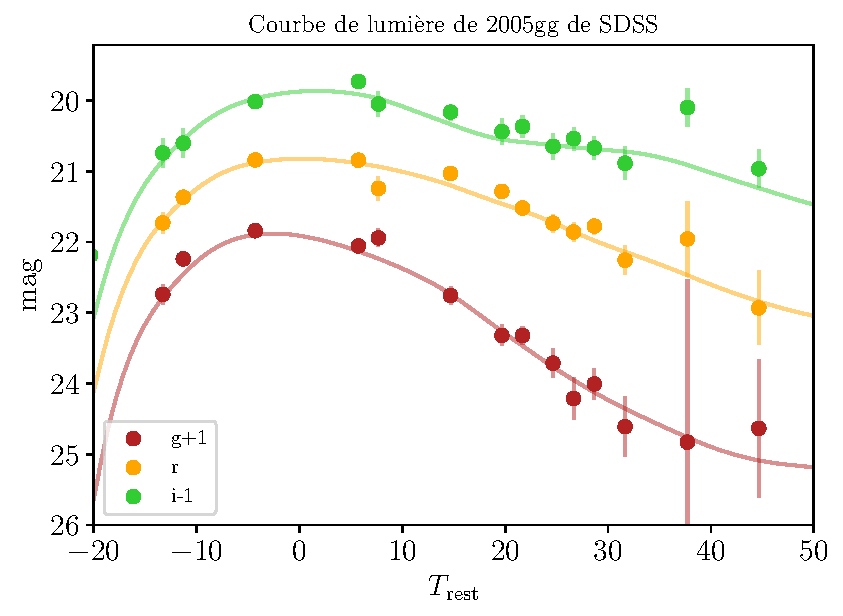
\includegraphics[width=.8\linewidth]{lc_2005gg.pdf}
%     \caption{Courbe de lumière en bandes $gri$ de la supernova SN 2005gg, une
%     SN Ia confirmée à $z = 0,230$. Le temps est compté en jours relativement au
% pic d'émission en bande $g$. Figure reproduite de~\cite{frieman2008}.}
%     \label{fig:sdsslc}
% \end{figure}

Pour discriminer entre bruit de fond et réelle variation astronomique, une
inspection visuelle par un humain était systématiquement nécessaire jusqu'en
2006, \textit{via} une interface web comportant les images dans les filtres
$gri$ et d'autres informations pertinentes. Des 5 filtres utilisés, ce sont donc
ces trois-là qui forment les meilleures mesures. Après cette date, la détection
est en partie laissée au logiciel \textit{autoscanner}. Sur les trois saisons
d'observation, ce sont 10258 nouveaux objets transitoires qui ont été
découverts.

\subsection{Suivi spectrophotométrique}\label{ssec:sdssspectro}

Le typage de SDSS utilise de nombreux différents télescopes~: le HET de
\SI{9,2}{m} \citep{hill1998}, le
ARC\footnote{\href{http://www.apo.nmsu.edu/arc35m/Instruments/DIS/\#B}
{http://www.apo.nmsu.edu/arc35m/Instruments/DIS/\#B}} de \SI{3,5}{m}, Subaru de
\SI{8,2}{m} \citep{kashikawa2000}, le
WHT\footnote{\href{http://www.ing.iac.es/PR/wht_info/whtisis.html}
{http://www.ing.iac.es/PR/wht\_info/whtisis.html}} de \SI{4,2}{m}, le
MDM\footnote{\href{http://www.astronomy.ohio-state.edu/MDM/CCDS/}
{http://www.astronomy.ohio-state.edu/MDM/CCDS/}} de \SI{2,4}{m}, le Keck de
\SI{10}{m} \citep{oke1995}, le
TNG\footnote{\href{http://www.tng.iac.es/instruments/lrs/}
{http://www.tng.iac.es/instruments/lrs/}} de \SI{3,5}{m}, le NTT de \SI{3,6}{m}
\citep{dekker1986}, le
NOT\footnote{\href{http://www.not.iac.es/instruments/alfosc/}
{http://www.not.iac.es/instruments/alfosc/}} de \SI{2,5}{m}, les télescopes de
\textit{Magellan}\footnote{\href{http://www.lco.cl/magellan-telescopes/}
{http://www.lco.cl/magellan-telescopes/}} de \SI{6,5}{m} et le SALT de
\SI{11}{m} \citep{burgh2003}. Plusieurs de ces télescopes pouvaient être prévus
pour observation la même nuit, rendant au total le temps alloué à la
spectroscopie supérieur au temps alloué à l'acquisition optique, permettant
l'acquisition de tous les candidats à $z \lesssim 0,15$.

Cependant, le nombre de candidats par nuit excède largement les capacités de
suivi spectroscopique, obligeant les opérateurs à faire une sélection des cibles
à analyser. Ainsi, une vérification visuelle a également été réalisée en
comparant les courbes de lumière dans les bandes $gri$ avec des librairies de
différents modèles pour en estimer les paramètres (redshift, date du maximum de
flux, magnitude apparente, contamination galactique…) et permettre de prioriser
les cibles à suivre spectroscopiquement. Notamment, les SNe~Ia les plus
prioritaires sont celles qui sont bien séparées du centre galactique ($\gtrsim
\ang{;;1}$), avec un contraste de luminosité SN/galaxie raisonnable (critère
visuel), et dont la galaxie hôte est relativement rouge. Le sondage requiert
généralement deux détections avant le suivi spectroscopique, mais par manque de
candidats à bas redshift ce critère a pu être réduit, contrairement aux données
à $z \gtrsim 0,2$ où les candidats ne manquent pas. L'algorithme choisi par SDSS
se rapproche fortement de celui du sondage SNLS, cf Section~\ref{sec:snls}.

En combinant les trois saisons d'observation, la phase II de SDSS a
spectroscopiquement confirmé 499 SNe~Ia \citep{sako2018}.

\subsection{Données conservées}\label{ssec:sdssdata}

Après l'acquisition des données, une sélection supplémentaire s'applique pour ne
retenir que les données dites « cosmologiques », c'est-à-dire qui correspondent
aux exigences de qualité pour être insérées dans le diagramme de
\textsc{Hubble}. Pour SDSS, en appelant $T_{\rm rest}$ le temps en jours par
rapport au maximum d'émission en bande $B$, les critères sur les courbes de
lumière avancés dans~\cite{kessler2009b} sont les suivants~:

\begin{enumerate}
    \item Au moins 1 mesure avant $T_{\rm rest} < \SI{0}{jour}$~;
    \item Au moins 1 mesure après $T_{\rm rest} > \SI{10}{jours}$~;
    \item Au moins 5 mesures entre $-15 < T_{\rm rest} < \SI{60}{jours}$~;
    \item Au moins 1 mesure avec un rapport signal sur bruit > 5 en bande $g$,
        $r$ et $i$~;
    \item $\mathcal{P}_{\rm fit} > 0,001$, où $\mathcal{P}_{\rm fit}$ est la
        probabilité d'optimisation par degré de liberté donné par le programme
        \texttt{MLCS2K2}, similaire à \texttt{SALT2.4} (cf.
        Section~\ref{ssec:salt}).
\end{enumerate}
Dans l'analyse finale de~\cite{scolnic2018}, les données photométriques qui sont
considérées aberrantes ($>4\s$) sont retirées. Le nombre total de données
conservées est alors de 335. La Figure~\ref{fig:sdsshist} en présente les
histogrammes en redshift, étirement et couleur.

\begin{figure}[ht]
    \centering
    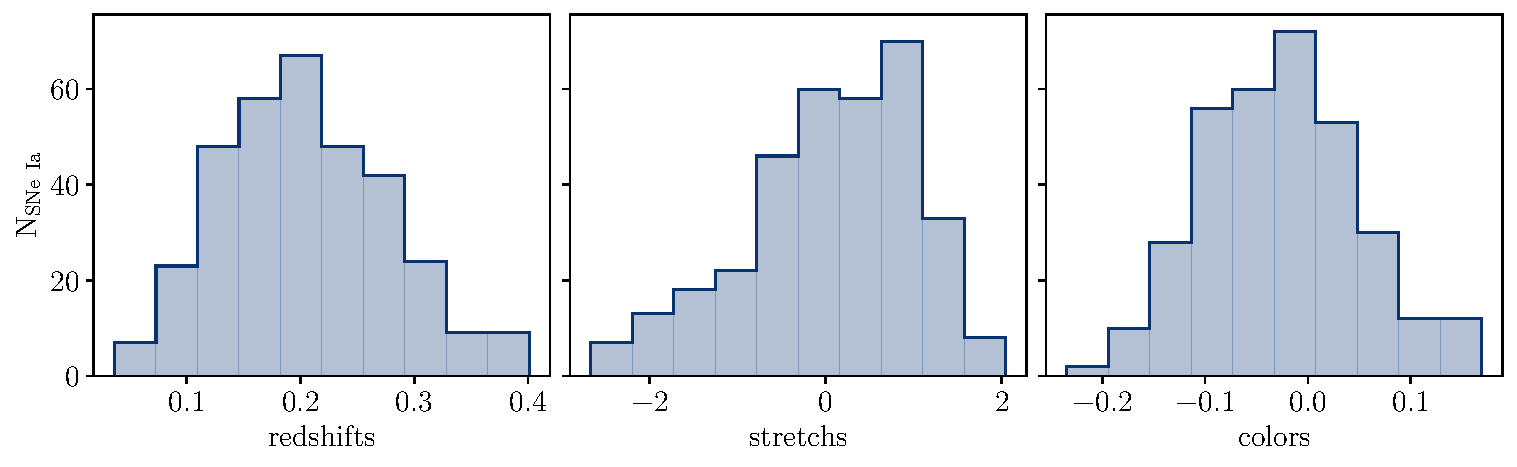
\includegraphics[width=\linewidth]{hist_SDSS_zxc.pdf}
    \caption[Distributions des paramètres de redshift, étirement et couleur de
    SDSS]{Distributions des paramètres de redshift (à gauche), d'étirement (au
    milieu) et de couleur (à droite) pour les 335 données de SDSS.}
    \label{fig:sdsshist}
\end{figure}

\section{Panoramic Survey Telescope and Rapid Response
System}\label{sec:ps1}

\subsection{Introduction}\label{ssec:ps1intro}

Le \textit{Panoramic Survey Telescope And Rapid Response System}
\citep[Pan-STARRS,][]{chambers2016, scolnic2018} est un site d'imagerie et de
traitement de données astronomiques à grand champ, dont le premier télescope,
PS1 (se confondant par la suite avec le nom du sondage) est situé au sommet du
Mont Haleakala sur l'île Maui de la chaîne d'îles hawaïenne. Son relevé a
commencé en 2009 pour se terminer en 2014. Son intervalle de redshifts sondés
s'étend de $0,02 < z < 0,65$, et ses objectifs scientifiques sont nombreux. Cela
inclut la photométrie de précision d'étoiles dans la Voie Lactée, le sondage du
système solaire avec recherche d'astres dangereux dans les environs de la Terre,
l'étude des phénomènes transitoires et la volonté de poser de nouvelles
contraintes sur l'énergie et la matière sombres. Ces deux derniers objectifs
sont ceux qui nous importent. 

\subsection{Détection des supernovae}\label{ssec:ps1detec}

Les relevés de PS1 sont réalisés grâce au sous-programme \textit{Medium Deep
Survey} (MDS) se concentrant sur 10 champs déjà bien étudiés de \SI{7}{deg^2}
chacun, pour une surface totale de \SI{70}{deg^2} et comptabilisant 25\% du
temps de PS1. Sa cadence est de 7 jours par filtre sur une période de 6 à
\SI{8}{mois} avec une profondeur de champ en bande $g$ de \SI{23,1}{mag}. Son
télescope \citep{hodapp2004} est composé d'un miroir primaire de \SI{1,8}{m} et
d'un secondaire de \SI{0,9}{m}, couplés à la \textit{Gigapixel Camera \#1}
\citep[GPC1,][]{kaiser2010, tonry2006} observant une zone du ciel de \ang{3,3;;}
de diamètre. Les observations s'effectuent par l'utilisation combinée de 5
filtres $grizy_{\rm P1}$. Ils sont globalement similaires à ceux de SDSS (voir
Section~\ref{sec:sdss}) à l'exception de la bande $g_{\rm P1}$ qui est
\SI{20}{nm} plus étendu du côté rouge du spectre et la bande $z_{\rm P1}$ qui a
une coupe plus nette à \SI{922}{nm}. Les transmissions des filtres sont tracées
Figure~\ref{fig:ps1bands}, et un exemple de courbe de lumière est présenté
Figure~\ref{fig:lc_550041}.

\begin{figure}[ht]
    \centering
    \begin{subfigure}[]{.49\linewidth}
        \centering
        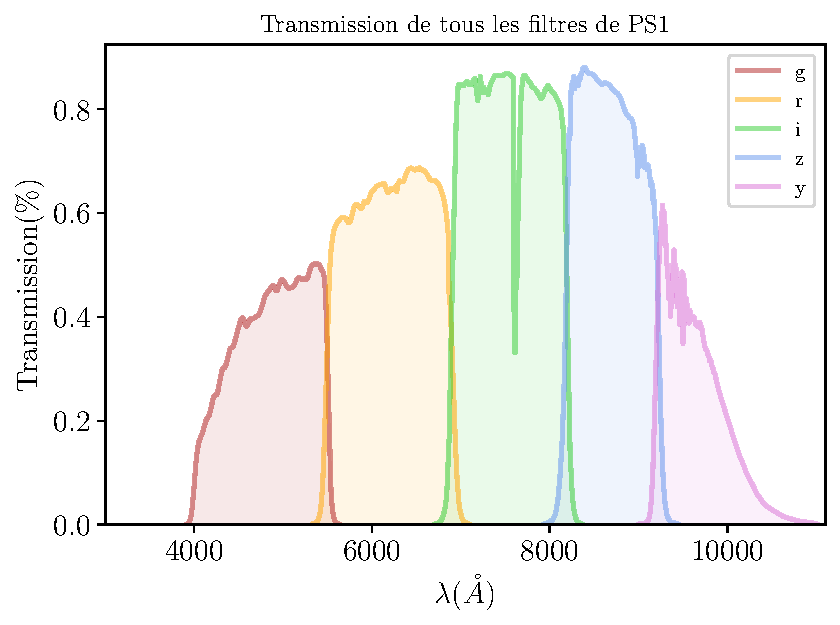
\includegraphics[width=\linewidth]{bands_PS1.pdf}
        \caption{Transmissions des filtres $grizy$ de la caméra utilisée par
        PS1. Données tirées du SVO \citep{rodrigo2020}.}
        \label{fig:ps1bands}
    \end{subfigure}
    \begin{subfigure}[]{.49\linewidth}
        \centering
        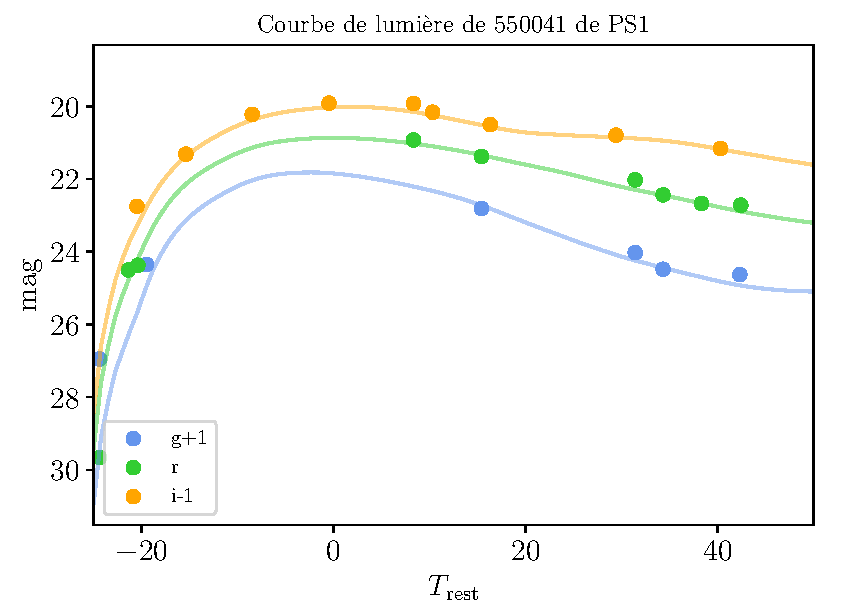
\includegraphics[width=\linewidth]{lc_550041.pdf}
        \caption{Courbe de lumière en bandes $gri$ de la SN Ia confirmée 550041,
        à $z = 0,26$.}
        \label{fig:lc_550041}
    \end{subfigure}
    \caption{Caractéristiques du sondage PS1.}
\end{figure}

\subsection{Suivi spectrophotométrique}\label{ssec:ps1spectro}

Comme SDSS, PS1 utilise de nombreux instruments pour le suivi
spectroscopique~: le \textit{Blue Channel Spectrograph} \citep{schmidt1989} et
le \textit{Hectospec} \citep{fabricant2005} sur le télescope MMT de \SI{6,5}{m},
les spectrographes de \textit{Gemini Multi-Object Spectrographs}
\citep[GMOS,][]{hook2004}, le \textit{Low Dispersion Survey Spectrograph-3}
(LDSS3\footnote{\href{http://www.lco.cl/telescopes-information/magellan/instruments-1/ldss-3-1}
{http://www.lco.cl/telescopes-information/magellan/instruments-1/ldss-3-1}}) et
le \textit{Magellan Echellette} \citep[MagE,][]{marshall2008} sur le télescope
\textit{Magellan Clay} de \SI{6,5}{m}, le \textit{Inamori-Magella Areal Camera
and Spectrograph} \citep[IMACS,][]{dressler2011} sur le télescope
\textit{Magellan Baade} de \SI{6,5}{m}, le spectrographe ISIS sur le
WHT\footnote{\href{http://www.ing.iac.es/PR/wht_info/whtisis.html}
{http://www.ing.iac.es/PR/wht\_info/whtisis.html}} de \SI{4,2}{m}, et le DEIMOS
\citep{faber2003} sur le Keck de \SI{10}{m} \citep{oke1995}.

Les critères les plus importants pour la sélection de candidats à observer
spectroscopiquement sont la position et la luminosité~: \textit{Magellan} et
\textit{Gemini} ne peuvent pointer que 5 des 10 champs du MDS, et certains
appareils ne peuvent acquérir des données qu'à $r_{\rm P1} \lesssim
\SI{21,5}{mag}$. La quantité de données observées par PS1 a souffert d'un manque
de maintenant et d'accès aux télescopes ainsi que du mauvais temps, réduisant
l'efficacité de suivi. L'évolution de ce paramètre en fonction de la magnitude
est discutée dans le chapitre suivant. En résumé, la limite de détection pour
identifier les phénomènes transitoires produit des courbes de lumière de qualité
pour les SNe~Ia de $m < 24$, alors que l'échantillon spectroscopique est
principalement constitué d'objets de $m < 22$. Au total, ce sont 365 SNe~Ia
confirmées qui constituent l'échantillon de PS1.

\subsection{Données conservées}\label{sec:ps1data}

Comme pour SDSS, pour une analyse cosmologique de qualité, chaque SN~Ia se doit
d'avoir une courbe de lumière bien échantillonnée afin de contraindre
correctement les paramètres d'optimisation et que ses propriétés
permettent de limiter les biais systématiques dans la distance finale.
Ainsi,~\cite{scolnic2018} utilisent les coupes suivantes~:
\begin{enumerate}
    \item Optimisation donnant $\chi^2/\mathrm{NDOF} < 3,0$ (avec NDOF le nombre
        de degrés de liberté), réduisant le sondage à 332 données~;
    \item Erreur sur $x_1$ ($\s_{x_1}$) $< 1,0$, laissant 303 SNe~Ia~;
    \item Erreur sur le pic de magnitude ($\s_{\rm pkmjd}$) $< 2,0$, ne causant
        aucune coupe~;
    \item Paramètre de couleur $c$ tel que $-0,3 < c < 0,3$, rejetant 10 SNe~Ia
        pour 293 restantes~;
    \item Paramètre d'étirement $x_1$ tel que $-3 < x_1 < 3$, que 5 SNe~Ia ne
        vérifient pas~;
    \item Extinction de la Voie Lactée $E(B-V)_{\rm MW}< \SI{0,20}{mag}$, ne
        s'appliquant pas aux données de PS1 grâce à la faible extinction des
        champs du MDS~;
    \item Au moins une mesure à $T_{\rm rest} > \SI{5}{jours}$, excluant 6
        SNe~Ia pour un total de 282 SNe~Ia.
\end{enumerate}
Une ultime coupe de l'analyse cosmologique par \textit{BEAMS with Bias
Correction} \citep[BBC,][]{kessler2017} réduit cet échantillon à 279 données. La
méthode BBC impose que les propriétés d'une SN se retrouvent dans les 99.999\%
d'un échantillon simulé de \num{500 000} SNe du même sondage~; en l'occurrence
les 3 SNe~Ia ne passant pas cette restriction ont pour paramètres $(x_1,c)$~:
$(−2,915, 0,083)$, $(−1,702, 0,271)$, et $(−0,893, 0,298)$. Ce procédé sera
discuté Chapitre~\ref{ch:snana}. Le Tableau~\ref{tab:ps1cuts} résume cette
sélection, et la Figure~\ref{fig:ps1hist} présente les histogrammes en
redshifts, étirement et couleur de ces 279 données.

\begin{table}[]
    \centering
        \caption{Critères de sélection des SNe~Ia suivies par PS1.}
        \label{tab:ps1cuts}
    \begin{threeparttable}
        \makebox[\linewidth]{%
        \begin{tabular}{lc}
            \toprule
            Critères de sélection     & Nb de SNe~Ia \\
            \midrule
            Confirmées                & 365 \\
            Courbe de lumière         & 332 \\
            $\s_{x_1} < 1$            & 303 \\
            $\s_{\rm pkmjd} < 2$      & 303 \\
            $-0,3 < c < 0,3$          & 293 \\
            $-3 < x_1 < 3$            & 288 \\
            $E(B-V)_{\rm MW} < 0,20 $ & 288 \\
            $T_{\max} > 5$            & 282 \\
            \midrule
            Coupe par BBC             & 279 \\
            \bottomrule
    \end{tabular}}
        \begin{tablenotes}[flushleft]
        \item\small \textbf{\hspace{-3,2pt}Notes.} Le nombre de SNe est tiré de
            l'analyse de Pantheon \citep{scolnic2018}.
        \end{tablenotes}
    \end{threeparttable}
\end{table}

\begin{figure}[ht]
    \centering
    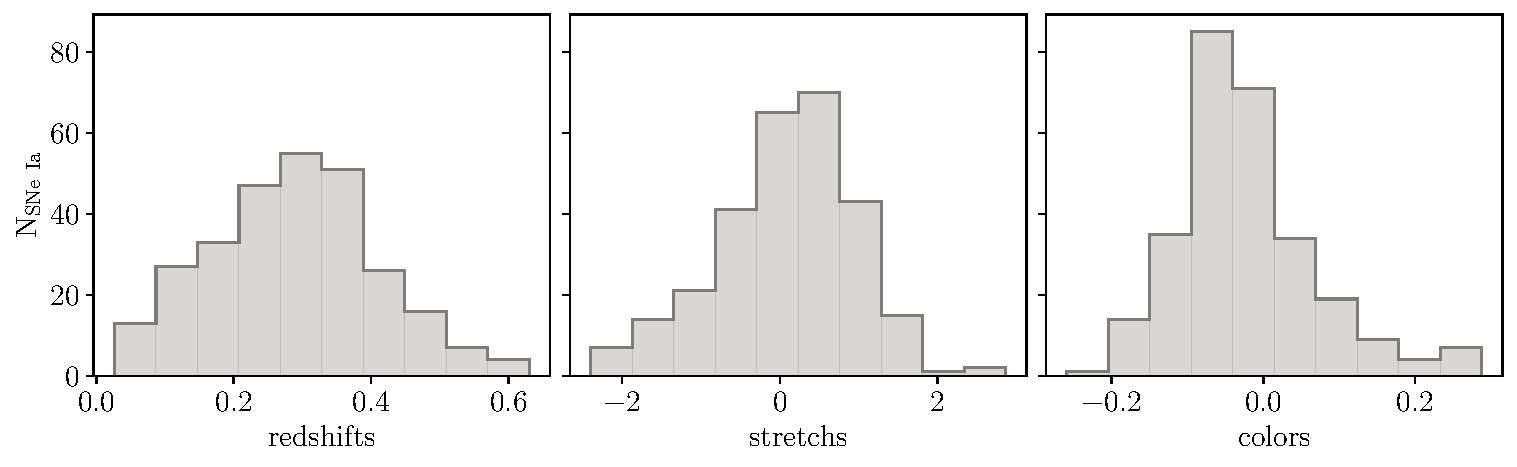
\includegraphics[width=\linewidth]{hist_PS1_zxc.pdf}
    \caption[Distributions des paramètres de redshift, étirement et couleur de
    PS1]{Distributions des paramètres de redshift (à gauche), d'étirement (au
    milieu) et de couleur (à droite) pour les 279 données de PS1.}
    \label{fig:ps1hist}
\end{figure}

\section{Supernova Legacy Survey}\label{sec:snls}
\subsection{Introduction}\label{ssec:snlsintro}

Le \textit{SuperNova Legacy Survey} \citep[SNLS,][]{astier2006, sullivan2011}
est un programme astronomique s'étendant sur 5 ans entre 2003 et début 2009,
dont le but principal est de mesurer l'expansion de l'Univers à l'aide de SNe~Ia
\textit{via} la mesure du paramètre d'état de l'énergie sombre $w$ à 5\% de
précision statistique et 10\% en incluant les effets systématiques. Il a été
conçu dans le but d'améliorer significativement les sondages passés grâce à sa
recherche glissante d'une part, mais également grâce à l'exploitation du service
d'observation à la fois pour la photométrie et la spectroscopie, réduisant
l'impact du mauvais temps. L'utilisation d'un seul instrument d'imagerie pour
observer les mêmes champs réduit les incertitudes systématiques photométriques.
L'observation de service optimise à la fois le rendement du temps d'observation
spectroscopique et l'échantillonnage de la courbe de lumière.

\subsection{Détection des supernovae}\label{ssec:snlsdetec}

SNLS utilise la caméra MegaCam \citep{boulade2003}, associée au télescope
Canada-France-Hawaï\footnote{\href{https://www.cfht.hawaii.edu/}
{https://www.cfht.hawaii.edu/}}, en se concentrant sur la partie profonde du
CFHTLS\footnote{\href{https://www.cfht.hawaii.edu/Science/CFHTLS/}
{https://www.cfht.hawaii.edu/Science/CFHTLS/}} représentant \SI{4}{deg^2} du
ciel réparti sur 4 champs de \SI{1}{deg^2} chacun et à faible extinction
galactique. L'acquisition se fait en 4 bandes $g'r'i'z'$ avec une cadence de
\SI{7}{jours} et une profondeur de \SI{25,0}{mag} en bande
$r$\footnote{\href{https://www.cfht.hawaii.edu/Science/CFHTLS/cfhtlsfinalreleaseexecsummary.html}
{https://www.cfht.hawaii.edu/Science/CFHTLS/cfhtlsfinalreleaseexecsummary.html}}
(et \SI{25,5}{mag} en bande $g$). Le système de filtre de SNLS est similaire à
celui de SDSS (cf. Section~\ref{sec:sdss}), les bandes $g$ et $i$ étant un peu
plus vers le rouge. Les quatre bandes de SNLS permettent au sondage mesurer la
couleur de toutes les SNe~Ia sur l'intervalle de redshifts sondés. En effet,
avec la distance les corrections $K$ deviennent notables, et la couleur est
définie \textit{via} la différence $B-V$ à bas redshift et $U-B$ à haut
redshift. Ceci s'effectue grâce à un contrôle de correspondance entre ces
mesures pour des SNe de redshift moyen combinant des mesures précises dans ces
quatre bandes. Les transmissions des filtres sont tracées
Figure~\ref{fig:snlsbands}, et un exemple de courbe de lumière est donné
Figure~\ref{fig:snlslc}

\begin{figure}[ht]
    \centering
    \begin{subfigure}[]{.49\linewidth}
        \centering
        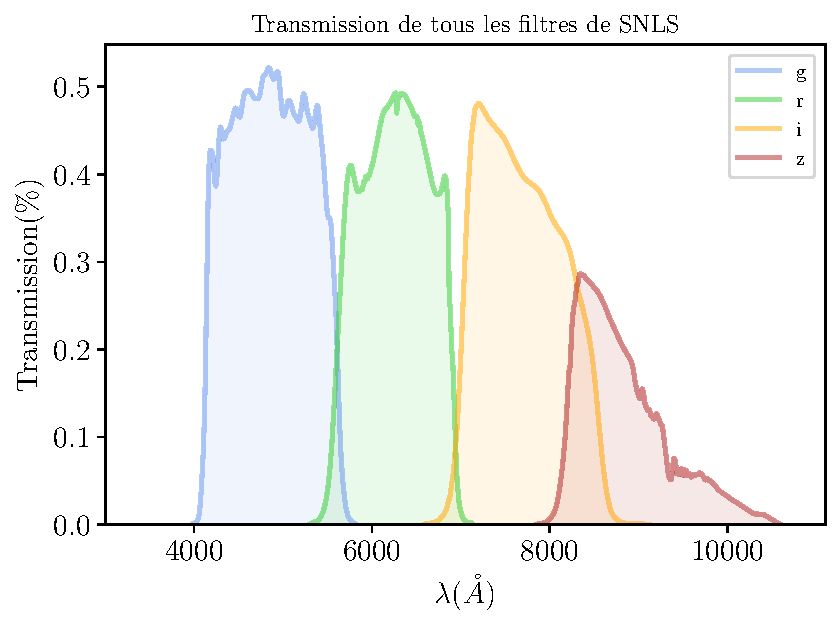
\includegraphics[width=\linewidth]{bands_SNLS.pdf}
        \caption{Transmissions des filtres de MegaCam utilisés par SNLS. Données
        tirées du SVO \citep{rodrigo2020}.}
        \label{fig:snlsbands}
    \end{subfigure}
    \begin{subfigure}[]{.49\linewidth}
        \centering
        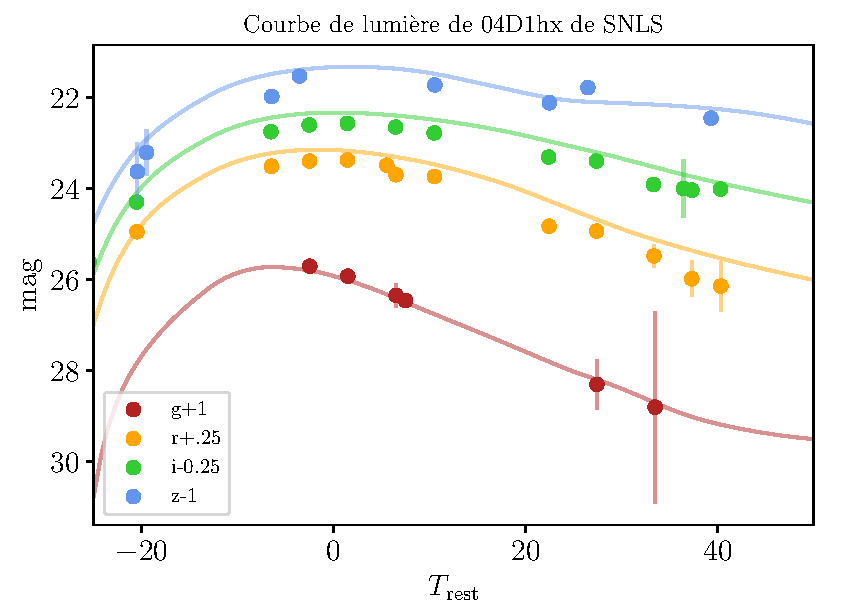
\includegraphics[width=\linewidth]{lc_04D1hx.pdf}
        \caption{Courbe de lumière en bandes $griz$ de la SN~Ia confirmée
        04D1hx, à $z = 0,56$. Figure produite avec les données du
        sondage et de l'analyse Pantheon \citep{scolnic2018}.}
        \label{fig:snlslc}
    \end{subfigure}
    \caption{Caractéristiques du sondage SNLS.}
\end{figure}

\subsection{Suivi spectrophotométrique}\label{ssec:snlsspectro}

Par la profondeur de son acquisition, SNLS utilise des télescopes dont les
miroirs ont un diamètre entre 8 et \SI{10}{m}~: le Keck \citep{oke1995,
ellis2008}, le Very Large Telescope \citep[VLT,][]{balland2009} et les
télescopes Gemini \citep{hook2004} pour le typage et la détermination du
redshift. Toutes les données de SNLS doivent être confirmées
spectroscopiquement. La partie photométrique du sondage délivrant plus de
candidats qu'il n'est possible d'observer spectroscopiquement, un classement des
phénomènes transitoires a dû être effectué. Ce classement est déterminé en vue
d'optimiser le rendement en SNe~Ia, et utilise à la fois un outil de sélection
photométrique réalisant un ajustement de courbe de lumières en temps réel pour
éviter la contamination avec d'autres types de SNe~Ia, mais aussi
une base de données de tous les phénomènes transitoires observés pour écarter
les étoiles variables qui varient sur des temps longs (plus d'une année). Les
candidats les moins lumineux, $i > \SI{24,5}{mag}$ (probablement à $z > 1$) et
ceux dont la luminosité n'est que faiblement supérieure à celle de leur galaxie
hôte (complexifiant l'identification) ne sont pas observés~: avec cette méthode,
environ 70\% des candidats observés se sont avérés être des SNe~Ia
\citep{astier2006}. Sur la totalité de l'existence de ce sondage, ce sont 242
supernovae qui ont été suivies et confirmées.

\subsection{Données conservées}\label{sec:snlsdata}

Toujours suivant~\cite{scolnic2018}, les données conservées répondent aux coupes
mentionnées Section~\ref{sec:ps1}, les mêmes que pour PS1. L'échantillon final
se compose alors de 236 SNe~Ia. Une présentation graphique des données en
redshift, étirement et couleur de ces données est présentée
Figure~\ref{fig:snlshist}.

\begin{figure}[ht]
    \centering
    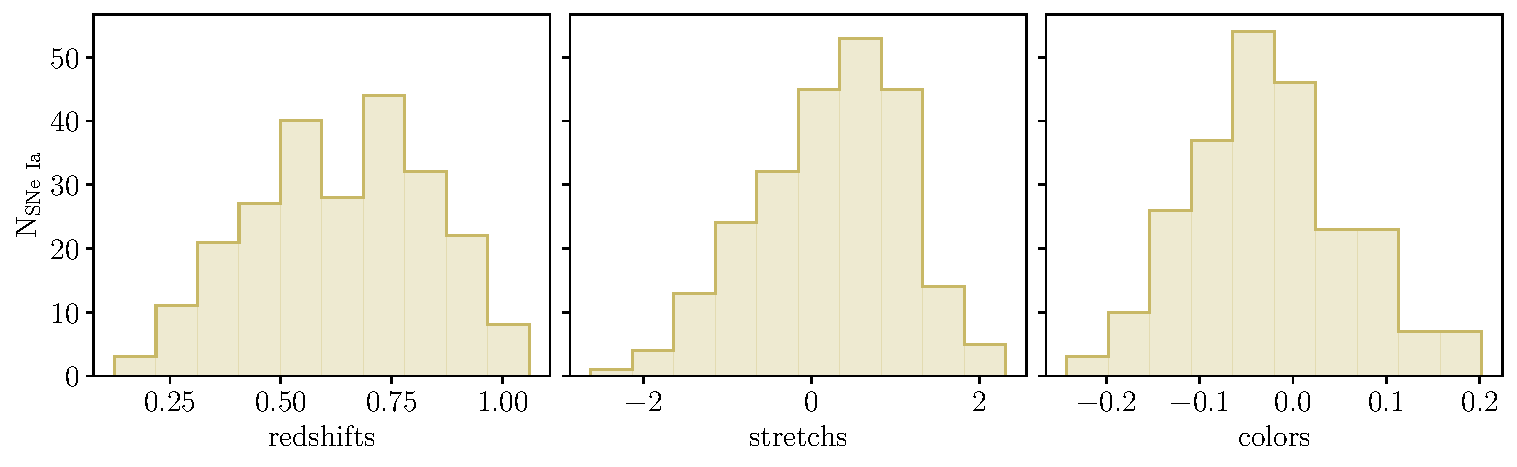
\includegraphics[width=\linewidth]{hist_SNLS_zxc.pdf}
    \caption[Distributions des paramètres de redshift, étirement et couleur de
    SNLS]{Distributions des paramètres de redshift (à gauche), d'étirement (au
    milieu) et de couleur (à droite) pour les 236 données de SNLS.}
    \label{fig:snlshist}
\end{figure}

\section{\textsc{Hubble} Space Telescope}\label{sec:hst}

Plusieurs sondages permettant l'acquisition de données de SNe~Ia ont été
effectués avec le télescope spatial \textsc{Hubble}
(HST\footnote{\href{https://www.nasa.gov/mission_pages/hubble/story/index.html}
{https://www.nasa.gov/mission\_pages/hubble/story/index.html}})~: le
\textit{Great Observatories Origins Deep
Survey} \citep[GOODS,][]{giavalisco2004, strolger2004, riess2007}, le
\textit{Supernova Cosmology Project} \citep[SCP,][]{suzuki2012}, et les sondages
\textit{Cosmic Assembly Near-infrared Deep Extragalactic Legacy
Survey} \citep[CANDELS,][]{rodney2014} et \textit{Cluster Lensing And Supernova
Survey with Hubble} \citep[CLASH,][]{graur2014}. Tous ces sondages recueillent
des données à $z > 1$ qui se révèlent d'une grande importance par leur poids
dans le diagramme de \textsc{Hubble} pour tester l'évolution des propriétés des
SNe. Ils sont combinés par la suite sous le nom «~HST~». Ainsi, par souci
d'efficacité, nous ne détaillons ici que les résultats issus de GOODS qui
constituent la plus grande part des données à haut redshift de notre
échantillon.

\subsection{Introduction}\label{ssec:hstintro}

Le sondage \textit{\textsc{Hubble} Higher $z$ Supernova
Search} \citep[HHZSS,][]{strolger2004}, sous-programme de GOODS, est un des
premiers sondages de recherche de SNe depuis l'espace. Son but principal est
d'étudier la présence de biais astrophysiques rendant les SNe~Ia intrinsèquement
moins lumineuses avec la distance, imitant une preuve de l'existence de
l'énergie sombre. Ce programme vise à relever des données au-delà de $z = 1$,
entre $1 < z < 2$. Dans cette plage, les SNe~Ia devraient exploser à une époque
de décélération cosmique, devenant ainsi relativement plus brillantes qu'à des
décalages vers le rouge plus faibles. On s'attend à ce que cela se distingue
clairement des simples effets de mesure astrophysiques, permettant une meilleure
connaissance des SNe~Ia. Étudier de manière approfondie et fiable ces SNe~Ia et
réaliser les observations de suivi nécessaires pour une telle étude nécessite
des observations plus profondes que ce qui peut être réalisé avec des télescopes
terrestres. Les observations de ce sondage s'étendent sur une plage
\SI{8}{mois}.

\subsection{Détection des supernovae}\label{ssec:hstdetec}

Ce programme utilise la \textit{Advanced Camera for
Surveys}\footnote{\href{https://www.nasa.gov/content/hubble-space-telescope-advanced-camera-for-surveys}
{https://www.nasa.gov/content/hubble-space-telescope-advanced-camera-for-surveys}}
(ACS). GOODS combine des observations multibandes extrêmement profondes de
l'ultraviolet à l'optique (dans le référentiel au repos) par le biais des
filtres F435W, F606W, F775W et F850LP, avec une magnitude limite pour F850LP
$\approx$ 26. Deux champs ont été observés pour une surface totale d'acquisition
de \SI{300}{arcmin^2}, chacun à haute latitude écliptique pour permettre aux
opérations au sol d'observer depuis les deux hémisphères. Sa cadence est
d'environ \SI{45}{jours}, suffisante pour détecter les SNe~Ia vers le maximum
d'émission pour $z \approx 1$ et avant le maximum pour $z > 1,3$, dû à
l'étalement de la courbe de lumière du fait de l'expansion (dans le référentiel
au repos le temps de montée typique est de $\approx \SI{20}{jours}$). Elle
permet également de s'assurer qu'une SN dépassant le seuil de détection ne
repasse pas en-dessous avant la seconde observation. Les transmissions des
filtres utilisés par le sondage sont tracées Figure~\ref{fig:hstbands}.

\begin{figure}[!ht]
    \centering
    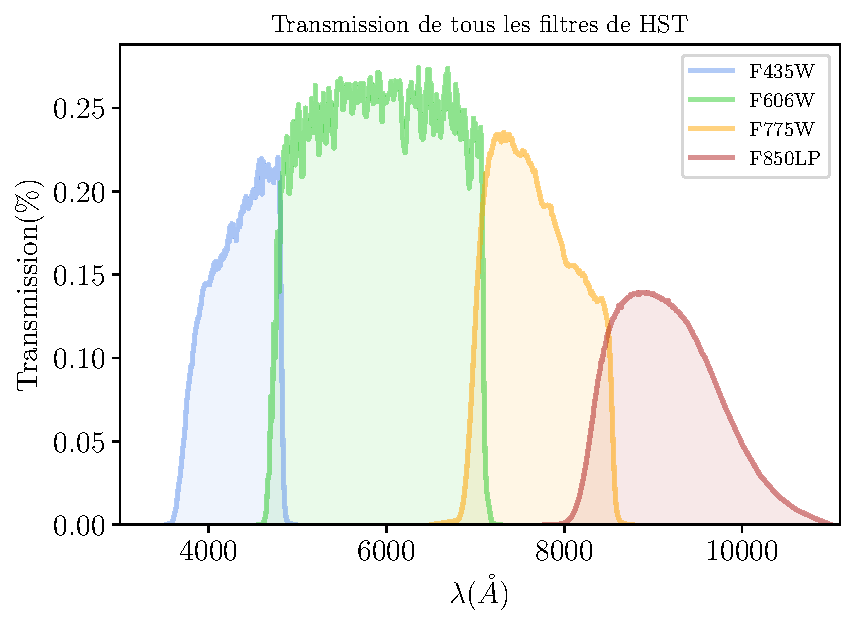
\includegraphics[width=.6\linewidth]{bands_HST.pdf}
    \caption[Transmissions des filtres de la caméra du sondage HST]
    {Transmissions des filtres de ACS utilisés par HST. Données tirées du SVO
    \citep{rodrigo2020}.}
    \label{fig:hstbands}
\end{figure}

\subsection{Suivi spectrophotométrique}\label{ssec:hstspectro}

Le HST, grâce à sa présence dans l'espace notamment, permet de produire des
spectres avec un rapport signal sur bruit significativement supérieur à ce qu'il
est possible d'atteindre par rapport à un instrument au sol. Il est cependant
limité par sa faible résolution spectrale et le recouvrement de multiples ordres
spectraux d'autres sources proches~: ainsi, seules les SNe avec une séparation
angulaire notable d'avec leur hôte et d'autres sources lumineuses ont été
observées. Une méthode secondaire d'identification des SNe~Ia par photométrie a
été utilisée pour optimiser la confirmation spectroscopique. \cite{riess2007}
détaillent les données ayant la plus haute qualité, qualifiées de «~dorées~»~:
celles dont la classification est certaine (rapport signal sur bruit $\gtrsim$
20) et dont la photométrie est suffisante pour amener à une estimation de
distance robuste, facilement caractérisée par les erreurs de mesure. On relève
42 données de~\cite{strolger2004} et 21 de~\cite{riess2007}.

\subsection{Données conservées}\label{ssec:hstdata}

À ces distances, le typage peut s'avérer difficile mais la classification des
données «~dorées~» est suffisamment robuste pour les inclure dans l'analyse
cosmologique de \citep{scolnic2018}~; ces données ne sont donc pas sujettes à
d'autres coupes. En combinant SCP, GOODS, CLASH et CANDELS, ce sont 26 données
qui constituent l'échantillon HST. Le détail des données par sondage est
indiqué Tableau~\ref{tab:hstcuts} et la distribution des paramètres en redshift,
étirement et couleur est montrée Figure~\ref{fig:hsthist}.

\begin{table}[]
    \centering
        \caption[Nombre de SNe~Ia de notre échantillon HST selon la
        source]{Nombre de SNe~Ia composant notre échantillon HST selon les
        sondages à haut redshifts.}
        \label{tab:hstcuts}
    \begin{threeparttable}
        \makebox[\linewidth]{%
        \begin{tabular}{lcc}
            \toprule
            Sondage & Nb de SNe~Ia & $z$ moyen \\
            \midrule
            SCP     & 3            & 1,092 \\
            GOODS   & 15           & 1,120 \\
            CLASH   & 2            & 1.555 \\
            CANDELS & 6            & 1,732 \\
            \midrule
            Total   & 26           & 1,278 \\
            \bottomrule
    \end{tabular}}
        \begin{tablenotes}[flushleft]
        \item\small \textbf{\hspace{-3,2pt}Notes.} Le nombre de SNe est tiré de
            l'analyse de Pantheon.
        \end{tablenotes}
    \end{threeparttable}
\end{table}

\begin{figure}[]
    \centering
    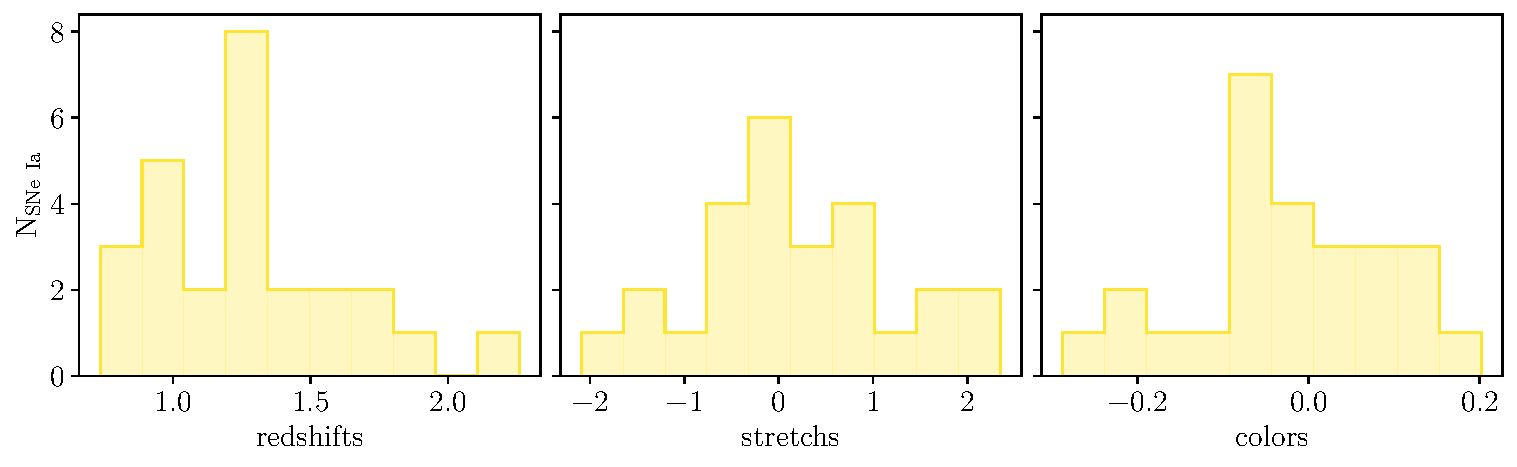
\includegraphics[width=\linewidth]{hist_HST_zxc.pdf}
    \caption[Distributions des paramètres de redshift, étirement et couleur de
    HST]{Distributions des paramètres de redshift (à gauche), d'étirement (au
    milieu) et de couleur (à droite) pour les 26 données de HST.}
    \label{fig:hsthist}
\end{figure}

\section{Autres sondages~: CfA1-4 et CSP}\label{sec:lowz}

Enfin, bien que ces sondages n'apparaissent pas dans la première partie de cette
étude, nous utilisons d'autres données à bas redshifts que celles issues de
SNfactory. Comme pour la section précédente, ces données proviennent d'une
combinaison de sondages~: celles des 4 relevés du \textit{Center for
Astrophysics} de Harvard, nommés CfA1 à 4 \citep{riess1999, jha2006,
hicken2009a, hicken2009b, hicken2012} et des 2 publications du \textit{Carnegie
Supernova Project} \citep[CSP,][]{contreras2010, folatelli2010,
stritzinger2011}. Ils ne feront pas l'objet de plus de détails étant donné que
ce sont tous les sondages à recherche ciblée que l'on écarte de notre
échantillon et qui n'interviendront que dans le Chapitre~\ref{ch:sims}. Cette
combinaison de sondages, résultant en 172 SNe~Ia après les coupes
de~\cite{scolnic2018}, est appelée \textit{LOWZ}, leurs données s'étalant entre
$0,01 < z < 0,07$. Une présentation de leurs distributions de paramètres en
redshift, étirement et couleur est cependant donnée Figure~\ref{fig:lowzhist}.

\begin{figure}[ht]
    \centering
    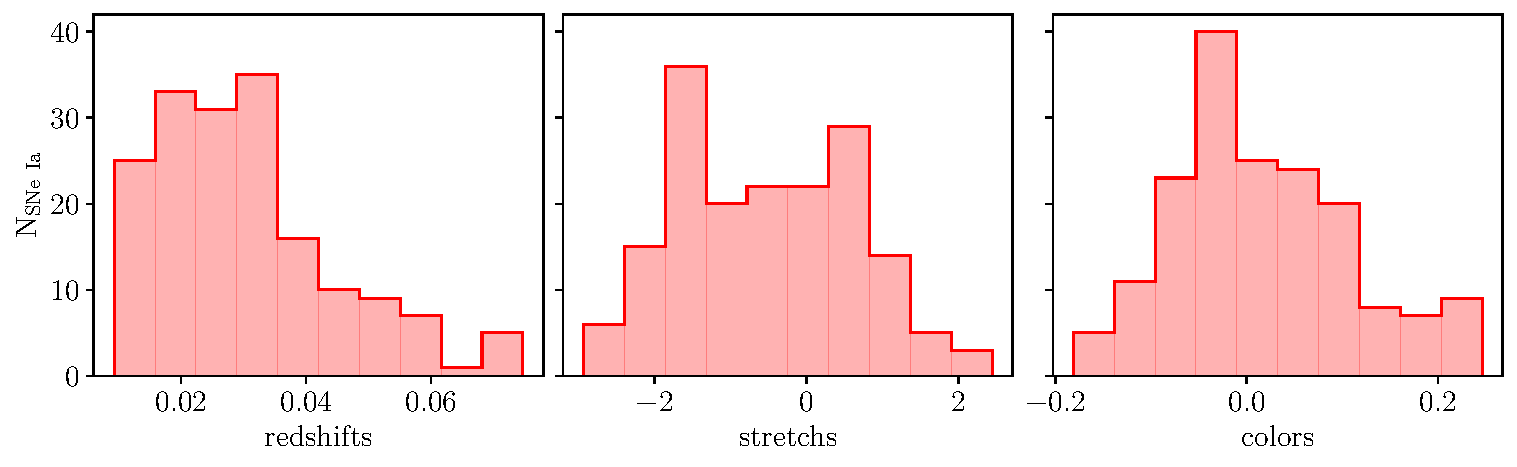
\includegraphics[width=\linewidth]{hist_LOWZ_zxc.pdf}
    \caption[Distributions des paramètres de redshift, étirement et couleur de
    LOWZ]{Distributions des paramètres de redshift (à gauche), d'étirement (au
    milieu) et de couleur (à droite) pour les 172 données de LOWZ.}
    \label{fig:lowzhist}
\end{figure}

\section{Complément~: Zwicky Transient Facility}\label{sec:ztf}
\subsection{Introduction}\label{ssec:ztfintro}

Le sondage de la \textit{Zwicky Transient Facility} \citep[ZTF,][]{bellm2019,
dekany2020} est un relevé cosmologique à grand champ qui a commencé ses
opérations en 2018. Comme d'autres sondages, plusieurs groupes de travail
composent ce relevé, tous participants à l'établissement de l'échantillon de
SNe~Ia. C'est le \textit{Bright Transient Survey} (BTS) qui y contribue en
majeure partie, la collaboration lui dédiant $\approx 80\%$ de son temps
d'observation total. L'échantillon acquit par ZTF se place comme le nouveau
sondage de référence à bas redshift, permettant de remplacer les données ciblées
des sondages CfA et CSP et l'utilisation d'instruments d'alerte extérieurs à la
collaboration de SNf par un seul échantillon homogène à recherche glissante.

Aux prémices de cette thèse, ces données n'étaient pas encore publiées, la
première phase ayant terminé en novembre 2020, et aujourd'hui ce sont les
résultats de la seconde phase qui sont en cours de production. C'est pourquoi
son implémentation n'est que limitée dans notre étude, et sert à discuter des
améliorations à la partie principale de notre travail, voir
Section~\ref{sec:xztf}.

\subsection{Détection des supernovae}\label{ssec:ztfdetec}

Le sondage utilise la caméra ZTF montée sur le télescope P48 Schmidt, à
l'Observatoire du Mont Palomar (comme SNf à l'époque, voir
Section~\ref{ssec:snfdetec}), et se concentre sur la partie nord du ciel. Son
champ de vision est de \SI{47}{deg^2}, le plus grand de tous les sondages
jusque-là, intègre 3 filtres $gri$ nommés ztf:g, ztf:r et ztf:i et a une cadence
moyenne de 3 jours tous champs et filtres confondus. Ses caractéristiques
uniques lui permettent de d'observer la totalité du ciel visible plus d'une fois
par nuit en moyenne avec une magnitude limite typique de \SI{20.5}{mag},
impliquant un rendu en SNe extrêmement élevé avec environ \num{1e5} alertes de
candidats par nuit. En moyenne, les données récoltées ont environ 10 points de
mesure avant le maximum d'émission, dont la médiane se situe à \SI{-13}{jours},
là où d'autres sondages manquent de données. Ceci permet une caractérisation
très efficace de l'étirement des SNe~Ia qui repose notamment sur
l'échantillonnage pré-explosion. Les transmissions des filtres sont présentées
Figure~\ref{fig:ztfbands} et un exemple de courbe de lumière produite
\textit{via} le module \texttt{ztfidr}
\footnote{\label{fn:ztfidr}\href{https://github.com/MickaelRigault/ztfidr}
{https://github.com/MickaelRigault/ztfidr}} est donné Figure~\ref{fig:ztflc}. 

\begin{figure}[ht]
    \centering
    \begin{subfigure}[]{.49\linewidth}
        \centering
        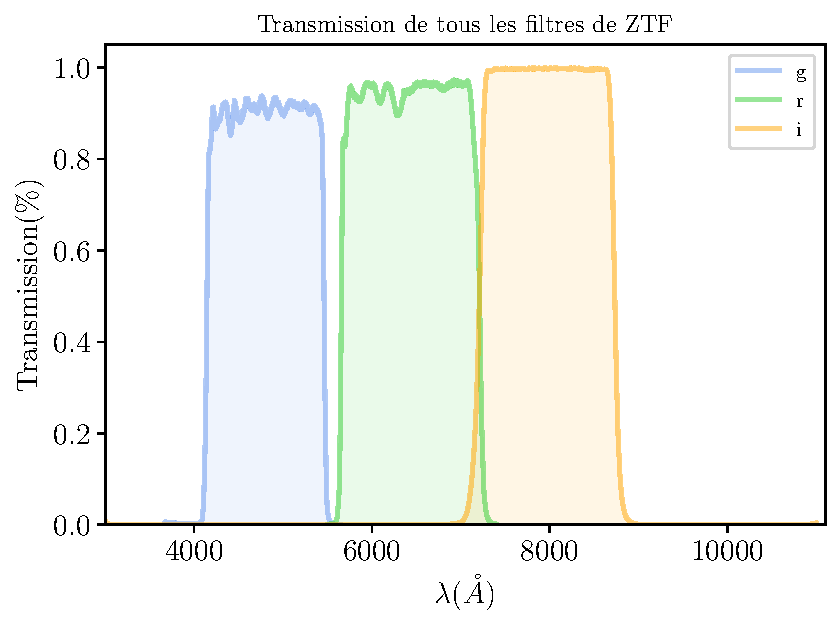
\includegraphics[width=\linewidth]{bands_ZTF.pdf}
        \caption[Transmissions des filtres de la caméra du sondage ZTF]
        {Transmissions des filtres de la caméra du sondage ZTF. Données tirées
        du SVO \citep{rodrigo2020}.}
        \label{fig:ztfbands}
    \end{subfigure}
    \begin{subfigure}[]{.49\linewidth}
        \centering
        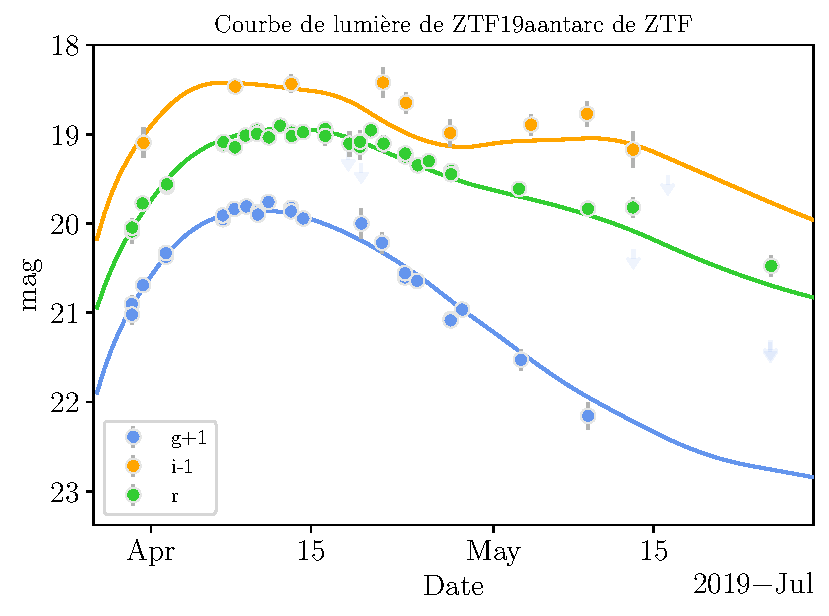
\includegraphics[width=\linewidth]{lc_ZTF19aantarc.pdf}
        \caption[Courbe de lumière de la SN ZTF19aantarc]{Courbe de lumière en
            bandes $gri$ de la SN~Ia confirmée ZTF19aantarc, à $z = 0,099$.
            Figure produite avec les données (à paraître) de la seconde
            publication du sondage \textit{via} le module
        \texttt{ztfidr}\footnoteref{fn:ztfidr}.}
        \label{fig:ztflc}
    \end{subfigure}
    \caption{Caractéristiques du sondage ZTF.}
\end{figure}

\subsection{Suivi spectrophotométrique}\label{ssec:ztfspectro}

À la différence des autres sondages, ZTF a un accès complet au spectrographe à
champ intégral \textit{SED machine} \citep[SEDm, voir][]{blagorodnova2018,
rigault2019} intégré au télescope P60, également au Mont Palomar. Par rapport au
SNIFS (Section~\ref{ssec:snfspectro}), le champ de vue passe de
$\ang{;;6.4}\times\ang{;;6.4}$ à $\ang{;;28}\times\ang{;;28}$ et la caméra de
guidage se voit dotée de 4 filtres $ugri$. Son objectif est d'acquérir tout
candidat transitoire de magnitude inférieure à \SI{18.5}{mag}. L'automatisation
de ce système permet une grande efficacité de détection et de suivi. Le sondage
travaille également avec le télescope P200 de \SI{5}{m} et le Keck de
\SI{10}{m}, et se verra prochainement accompagné d'une seconde SEDm sur un
télescope de \SI{2.5}{m} à Kitt Pick. Ainsi, des \num{1e5} alertes par nuit, ce
sont typiquement 7 qui sont des SNe~Ia. On compte à peu près 3700 SNe~Ia
spectroscopiquement confirmées dans les données de la seconde publication.

\subsection{Données conservées}\label{ssec:ztfdata}

Comme pour le reste des sondages, ZTF inclus des sélections supplémentaires sur
les données pour qu'elles soient de qualité «~cosmologique~». Leurs critères
sont les suivants~:
\begin{enumerate}
    \item Les données doivent provenir d'une image sans label indiquant une
        mauvaise qualité~;
    \item Seuls les points photométriques détectés à 5$\sigma$ sont considérés~;
    \item Au moins 7 mesures entre -15 < $T_{\rm rest}$ < \SI{30}{jours}~;
    \item Au moins 2 bandes avant et après le maximum d'émission parmi tous ces
        points.
\end{enumerate}
En plus de ces critères de qualité, l'échantillon retenu dans notre analyse suit
les sélections suivantes~:
\begin{enumerate}[resume]
    \item $-0,3 < c < 0,3$ et $\sigma_{c} < 0,3$~;
    \item $-3 < x_1 < 3$ et $\sigma_{x_1} < 1$.
\end{enumerate}
Ceux-ci assurent l'utilisation conjointe avec les autres sondages. Ainsi réduit,
ce sont 2246 SNe~Ia qui composent notre ensemble de données ZTF. La distribution
des paramètres de ces données en redshift, étirement et couleur est montrée
Figure~\ref{fig:ztfhist}.

\begin{figure}[]
    \centering
    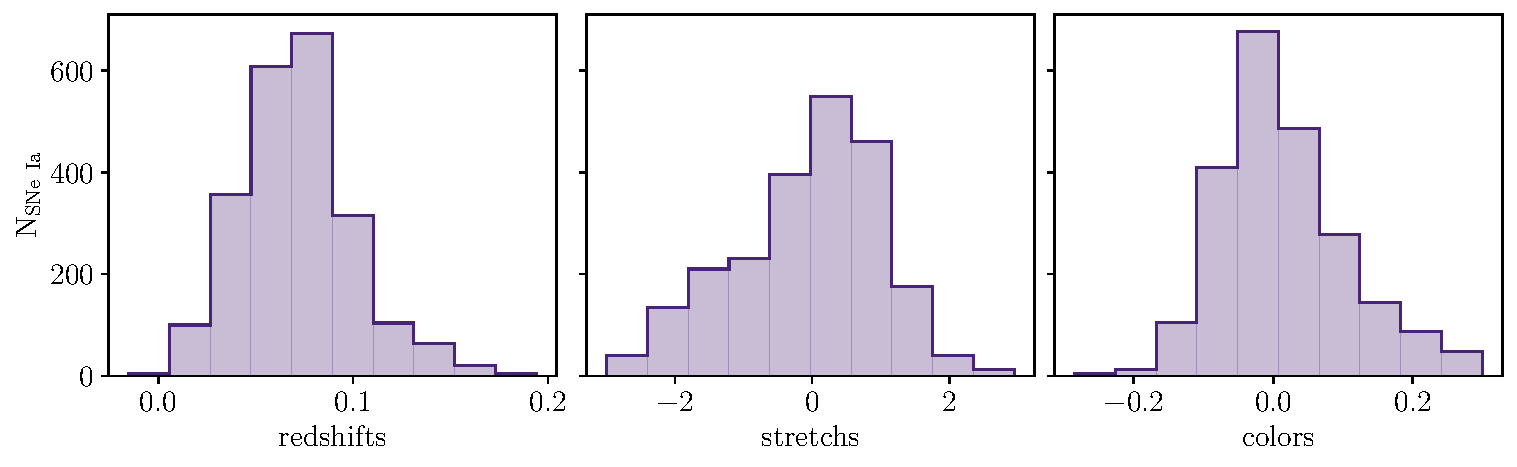
\includegraphics[width=\linewidth]{hist_ZTF_zxc.pdf}
    \caption[Distributions des paramètres de redshift, étirement et couleur de
    ZTF]{Distributions des paramètres de redshift (à gauche), d'étirement (au
    milieu) et de couleur (à droite) pour les 2246 données de ZTF.}
    \label{fig:ztfhist}
\end{figure}

\section{Résumé et comparaison}\label{sec:sondcomp}

Pour permettre une meilleure visualisation des diverses caractéristiques des
sondages traités dans cette thèse, nous donnons un graphique combiné des
distributions de tous les sondages Figure~\ref{fig:hist_all_zxc}, et présentons
Tableau~\ref{tab:sondcomp} une comparaison des éléments que nous considérons
comme principaux dans ces sondages.

\begin{figure}[ht!]
    \centering
    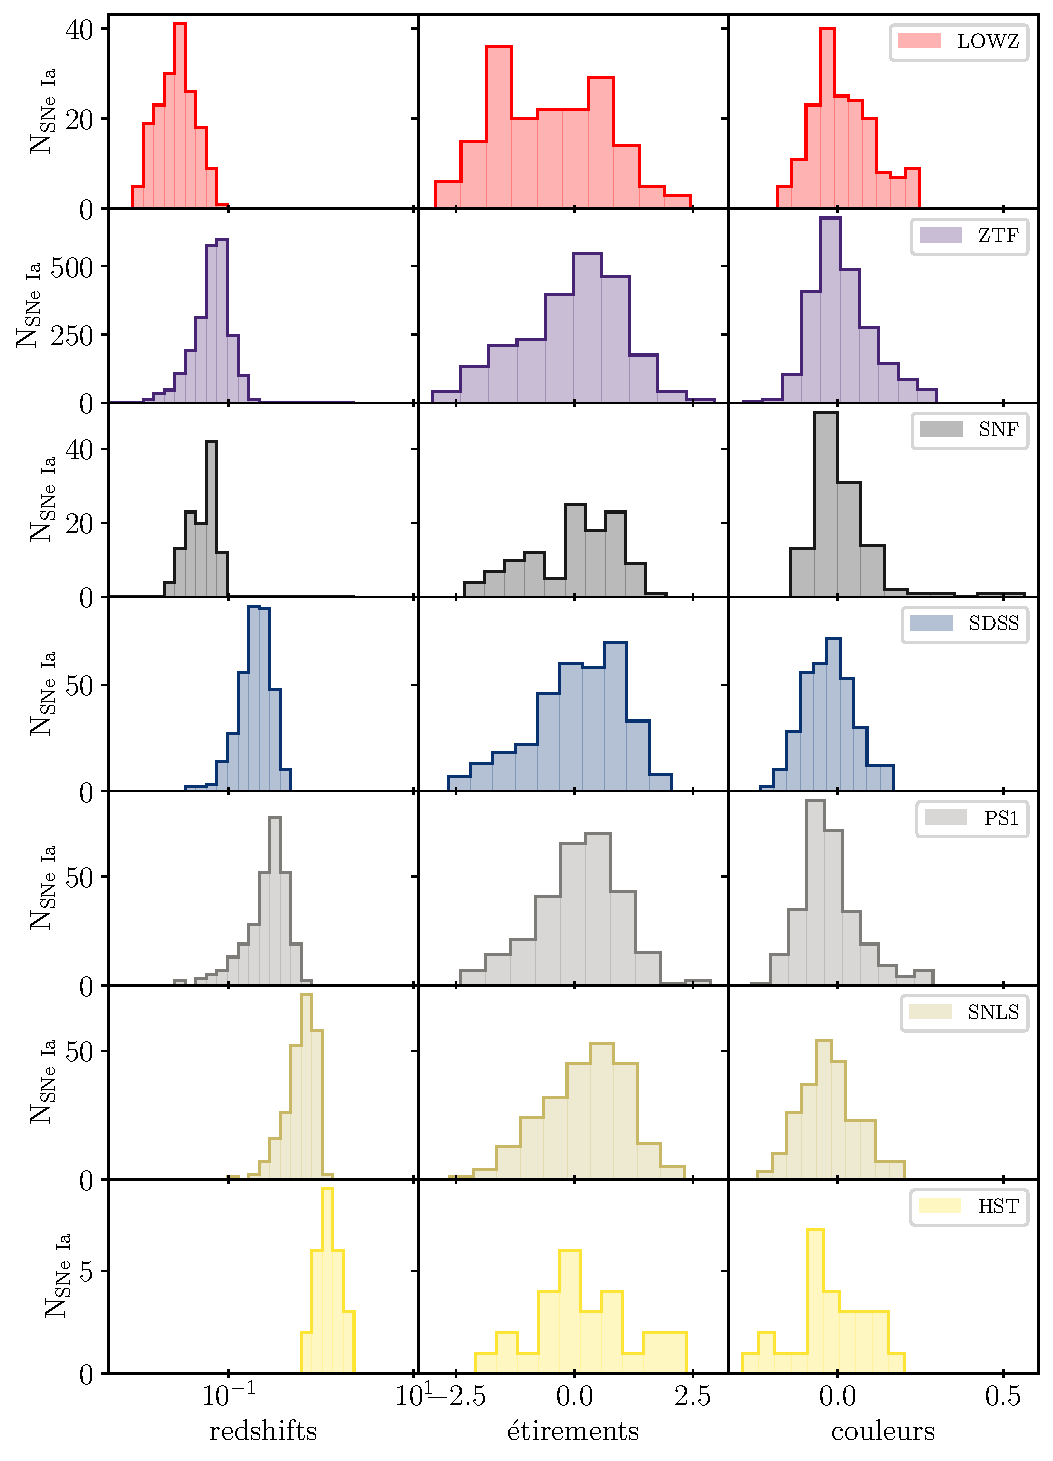
\includegraphics[width=.8\linewidth]{hist_all_zxc.pdf}
    \caption[Distributions des paramètres de redshift, étirement et couleur de
    tous les sondages utilisés dans cette étude]{Distributions des paramètres de
        redshift (à gauche), d'étirement (au milieu) et de couleur (à droite)
        pour tous les sondages utilisés dans cette étude. Le redshift est tracé
        en échelle logarithmique, nécessaire pour représenter des données à la
        fois riches à $z \lesssim 0,05$ et jusqu'à $z \approx 2$.}
    \label{fig:hist_all_zxc}
\end{figure}

Au travers des sections précédentes, nous avons pu avoir un aperçu de la
complexité que représentent les relevés cosmologiques. La variété des
intervalles de redshifts et donc des caractéristiques des sondages impose des
instruments variés, des stratégies spécifiques, mais également des calibrations
différentes. Travailler avec de nombreux pipelines d'analyse rend la combinaison
de sondages fastidieuse. C'est cet aspect que les prochains grands relevés
cosmologiques tentent d'améliorer~: le sondage \textit{Vera Rubin Observatory},
\textit{via} le \textit{Large Synoptic Survey Telescope}
\citep[LSST,][]{ivezic2019}, a pour objectif de couvrir un intervalle de
redshifts extrêmement grand, et le sondage de la \textit{Zwicky Transient
Facility} répond aux difficultés particulières de la partie à faible redshift de
la cosmologie, notamment l'ancrage de la valeur de H$_0$. À lui seul, il est
d'ores et déjà pratiquement deux fois plus grand que tous les autres sondages
réunis et représente le futur de la cosmologie basée sur les SNe~Ia.

\vfill
\shorthandoff{:}
\begin{table}[ht]
    \centerfloat
    \begin{threeparttable}
        \caption{Comparaison des caractéristiques des sondages utilisés.}
        \label{tab:sondcomp}
        \begin{tabular}{lcccccc}
            \toprule
            Sondage              &
            Surface (deg$^2$)    & Cadence (jours)   & Filtres          &
            Profondeur (mag)     & Intervalle $z$    & $N_{\rm SN}$\\
            \midrule
            \hyperref[sec:snf]{SNf}                      &
            500                      & 1                 & BV               &
            $r \lesssim 19,5$        & $0,02 < z < 0,08$ & 114\\
            \hyperref[sec:lowz]{LOWZ}\tnote{1}           &
            --                       & --                & $UBVRI$          &
            --                       & $0,01 < z < 0,07$ & 172\\
            \hyperref[sec:ztf]{ZTF}                      &
            Ciel nord                & 3                 & ztf:$gri$        &
            $r \lesssim 20,4$        & $0,00 < z < 0,19$ & 2246\\
            \hyperref[sec:sdss]{SDSS}                    &
            300                      & 4                 & $ugriz$          &
            $r \lesssim 22,5$        & $0,04 < z < 0,40$ & 335\\
            \hyperref[sec:ps1]{PS1}                      &
            70                       & 7                 & $grizy_{\rm P1}$ &
            $r \lesssim 23,1$        & $0,03 < z < 0,63$ & 279\\
            \hyperref[sec:snls]{SNLS}                    &
            4                        & 7                 & $g'r'i'z'$       &
            $r \lesssim 25,0$        & $0,13 < z < 1,06$ & 236\\
            \hyperref[sec:hst]{HST}\tnote{2}             &
            0,08                     & 45                & $griz$\tnote{3}  &
            F850LP $\lesssim 26$     & $0,74 < z < 2,26$ & 26\\
            \midrule
            Total & \multicolumn{5}{c}{} & 3408\tnote{4}\\
            \bottomrule
        \end{tabular}
        \begin{tablenotes}[flushleft]
        \item\small \textbf{\hspace{-3,2pt}Notes.} Le nombre de SNe est tiré de
            l'analyse de Pantheon.
        \item [1] \small  Caractéristiques non pertinentes en temps que sondages
            ciblés.
        \item [2] \small Caractéristiques pour GOODS, intervalle et nombre de
            SNe~Ia pour tous les sondages HST.
        \item [3] \small Relativement équivalent, cf. Figure~\ref{fig:hstbands}.
        \item [4] \small 990 sans LOWZ et ZTF, ce qui constitue la base de notre
            échantillon.
        \end{tablenotes}
    \end{threeparttable}
\end{table}
\shorthandon{:}
\vfill

\newpage

\thispagestyle{plain}
% \vspace*{-3cm}
\vfill
\minilof
\vfill
\minilot
\vfill

% \bibliographystyle{../main/aa_url}
% \shorthandoff{:}
% \bibliography{../chapters/99_references}

\end{document}
